%
%   Prof. Dr. Julian Reichwald
%   auf Basis einer Vorlage von Prof. Dr. Jörg Baumgart
%   DHBW Mannheim
%
%
%	ACHTUNG: Für das Erstellen des Literaturverzeichnisses wird das modernere Paket biblatex
%			 in Kombination mit biber verwenden -- nicht mehr das ältere BibTex!
% 			 Bitte stellen Sie ggf. Ihre TeX-Umgebung
% 			 entsprechend ein (z.B. TeXStudio: Einstellungen --> Erzeugen --> Standard Bibliographieprogramm: biber)
%

\documentclass[
	12pt,
	BCOR=5mm,
	DIV=12,
	headinclude=on,
	footinclude=off,
	parskip=half,
	bibliography=totoc,
	listof=entryprefix,
	toc=listof,
	pointlessnumbers,
	plainfootsepline]{scrreprt}

%	Konfigurationsdatei einziehen
% !TEX root =  master.tex

%		LANGUAGE SETTINGS AND FONT ENCODING 
%
\usepackage[ngerman]{babel} 	% German language
\usepackage[utf8]{inputenc}
\usepackage[german=quotes]{csquotes} 	% correct quotes using \enquote{}
\usepackage[T1]{fontenc}
\usepackage{lipsum}
\usepackage[colorlinks=false]{hyperref}
%\usepackage[english]{babel}   % For english language
%\usepackage{csquotes} 	% Richtiges Setzen der Anführungszeichen mit \enquote{}

% 		HYPERREF
%
% \usepackage[
% 	hidelinks=true % keine roten Markierungen bei Links
% ]{hyperref}


% Zwei eigene Befehle zum Setzen von Autor und Titel. Ausserdem werden die PDF-Informationen richtig gesetzt.
\newcommand{\TitelDerArbeit}[1]{\def\DerTitelDerArbeit{#1}\hypersetup{pdftitle={#1}}}
\newcommand{\AutorDerArbeit}[1]{\def\DerAutorDerArbeit{#1}\hypersetup{pdfauthor={#1}}}
\newcommand{\Firma}[1]{\def\DerNameDerFirma{#1}}
\newcommand{\Kurs}[1]{\def\DieKursbezeichnung{#1}}


% Correct superscripts 
\usepackage{fnpct}




%		CALCULATIONS
%
\usepackage{calc} % Used for extra space below footsepline



%		BIBLIOGRAPHY SETTINGS
%

% Uncomment the next three lines for author-year-style with footnotes (Chicago)
\usepackage[backend=biber, autocite=footnote, style=authoryear, dashed=false]{biblatex} 	%Use Author-Year-Cites with footnotes
\AdaptNoteOpt\footcite\multfootcite   %will add  separators if footcite is called multiple consecutive times 
\AdaptNoteOpt\autocite\multautocite % will add  separators if autocite is called multiple consecutive times

% Uncomment the next line for IEEE-style 
% \usepackage[backend=biber, autocite=inline, style=ieee]{biblatex} 	% Use IEEE-Style (e.g. [1])

% Uncomment the next line for alphabetic style 
% \usepackage[backend=biber, autocite=inline, style=alphabetic]{biblatex} 	% Use alphabetic style (e.g. [TGK12])

% Uncomment the next two lines vor Harvard-Style 
%\usepackage[backend=biber, style=apa]{biblatex} 	
%\DeclareLanguageMapping{german}{german-apa}


\DefineBibliographyStrings{ngerman}{  %Change u.a. to et al. (german only!)
	andothers = {{et\,al\adddot}},
}

%%% Uncomment the following lines to support hard URL breaks in bibliography 
%\apptocmd{\UrlBreaks}{\do\f\do\m}{}{}
%\setcounter{biburllcpenalty}{9000}% Kleinbuchstaben
%\setcounter{biburlucpenalty}{9000}% Großbuchstaben


\setlength{\bibparsep}{\parskip}		%add some space between biblatex entries in the bibliography
\addbibresource{bibliography.bib}	%Add file bibliography.bib as biblatex resource


%		FOOTNOTES 
%
% Count footnotes over chapters
\usepackage{chngcntr}
\counterwithout{footnote}{chapter}


%	ACRONYMS
%%%
%%% WICHTIG: Installieren Sie das neueste Acronyms-Paket!!!
%%%
\makeatletter
\usepackage[printonlyused]{acronym}
\@ifpackagelater{acronym}{2015/03/20}
  {%
    \renewcommand*{\aclabelfont}[1]{\textbf{\textsf{\acsfont{#1}}}}
  }%
  {%
  }%
\makeatother

%		LISTINGS
\usepackage{color}
\usepackage{listings}	%Format Listings properly
% Color
\definecolor{Gray}{RGB}{119, 162, 247}
\definecolor{Blue}{RGB}{209, 227, 255}
\definecolor{DarkBlue}{RGB}{38, 58, 209}
\definecolor{Green}{RGB}{184, 255, 222}
\definecolor{Red}{RGB}{255, 206, 184} 
\definecolor{DarkPurple}{rgb}{0.4,0.2,0.6}
\definecolor{GreenCom}{rgb}{0.3,0.5,0.3} 
\definecolor{OrangeString}{RGB}{212, 158, 21}
 
% \makeatletter
% \providecommand\phantomcaption{\caption@refstepcounter\@captype}
% \makeatother

\renewcommand{\lstlistingname}{Quelltext} 
\renewcommand{\lstlistlistingname}{Quelltextverzeichnis}
\lstset{numbers=left,
  numberstyle=\tiny,
  language=Java,
  frame=single,
    captionpos=b,
  basicstyle=\ttfamily\small,
  keywordstyle=\bfseries\color{DarkBlue},
  commentstyle=\itshape\color{GreenCom},
  stringstyle=\color{OrangeString},
  aboveskip=30pt,
  belowskip=30pt,
  breaklines=true
}

%		EXTRA PACKAGES
\usepackage{scrextend}
\usepackage{subfig}
\usepackage{lipsum}    %Blindtext
\usepackage{graphicx} % use various graphics formats
\usepackage[german]{varioref} 	% nicer references \vref
\usepackage{caption}	%better Captions
\usepackage{booktabs} %nicer Tabs
\usepackage{array}
\usepackage[T1]{fontenc}
\usepackage{amssymb}
\usepackage{algcompatible}
\usepackage{mwe}    % loads »blindtext« and »graphicx«
% \usepackage{subfig}
% \usepackage{unicode-math}
% \usepackage{algorithmicx}
% \usepackage{algpseudocode}

%\newcolumntype{P}[1]{>{\raggedright\arraybackslash}p{#1}}


		% ALGORITHMS
\usepackage{algorithm}
\usepackage{algpseudocode}
% \usepackage{algorithm,algpseudocode}
\renewcommand{\listalgorithmname}{Algorithmenverzeichnis }
\floatname{algorithm}{Algorithmus}


%		FONT SELECTION: Entweder Latin Modern oder Times / Helvetica
\usepackage{lmodern} %Latin modern font
%\usepackage{mathptmx}  %Helvetica / Times New Roman fonts (2 lines)
%\usepackage[scaled=.92]{helvet} %Helvetica / Times New Roman fonts (2 lines)

%		PAGE HEADER / FOOTER
%	    Warning: There are some redefinitions throughout the master.tex-file!  DON'T CHANGE THESE REDEFINITIONS!
\RequirePackage[automark,headsepline,footsepline]{scrpage2}
\pagestyle{scrheadings}
\renewcommand*{\pnumfont}{\upshape\sffamily}
\renewcommand*{\headfont}{\upshape\sffamily}
\renewcommand*{\footfont}{\upshape\sffamily}
\renewcommand{\chaptermarkformat}{}
\RedeclareSectionCommand[beforeskip=0pt]{chapter}
\clearscrheadfoot

\ifoot[\rule{0pt}{\ht\strutbox+\dp\strutbox}DHBW Mannheim]{\rule{0pt}{\ht\strutbox+\dp\strutbox}DHBW Mannheim}
\ofoot[\rule{0pt}{\ht\strutbox+\dp\strutbox}\pagemark]{\rule{0pt}{\ht\strutbox+\dp\strutbox}\pagemark}

\ohead{\headmark}


\begin{document}

%% BITTE GEBEN SIE HIER DEN TITEL UND DIE AUTORIN / DEN AUTOR DER ARBEIT AN!
%% DIESE INFORMATIONEN _MÜSSEN_ GESETZT SEIN, UM TITELBLATT, ABSTRACT UND
%% EIGENSTÄNDIGKEITSERKLÄRUNG AUTOMATISCH ANZUPASSEN!
\TitelDerArbeit{Variation, Analyse und Verbesserung eines Algorithmus zur heuristischen Lösung des Travelling Salesman Problems}
\AutorDerArbeit{Benno Grimm}
\Firma{SAP SE}
\Kurs{WWI18SEA}

\begin{titlepage}
\begin{minipage}{\textwidth}
		\vspace{-2cm}
		\noindent 
\includegraphics[scale=0.14]{img/firmenlogo.jpg} \hfill   
\includegraphics{img/logo.jpg}
\end{minipage}
\vspace{1em}
\sffamily
\begin{center}
	\textsf{\large{}Duale Hochschule Baden-W\"urttemberg\\[1.5mm] Mannheim}\\[2em]
	\textsf{\textbf{\Large{}Projektarbeit I}}\\[3mm]
	\textsf{\textbf{\DerTitelDerArbeit}} \\[1.5cm]
	\textsf{\textbf{\Large{}Studiengang Wirtschaftsinformatik}\\[3mm] \textsf{Studienrichtung Software Engineering}}
	
	\vspace{3em}
	%\textsf{\Large{Sperrvermerk}}
\vfill

\begin{minipage}{\textwidth}

\begin{tabbing}
	Wissenschaftlicher Betreuer: \hspace{0.85cm}\=\kill
	Verfasser/in: \> Benno Grimm \\[1.5mm]
	Matrikelnummer: \> 5331201 \\[1.5mm]
	Firma: \> SAP SE  \\[1.5mm]
	Abteilung: \> Transportation Management \\[1.5mm]
	Kurs: \> WWI18SEA \\[1.5mm]
	Studiengangsleiter: \> Prof. Dr. Julian Reichwald  \\[1.5mm]
	Wissenschaftlicher Betreuer: \> Prof. Dr. Julian Reichwald \\
	\> julian.reichwald@dhbw-mannheim.de \\
	\> +49 (0)621 4105 - 1395 \\[1.5mm]
	Firmenbetreuer: \> Peter Wadewitz \\
	\> peter.wadewitz@sap.com \\
	\> +49 6227 7-63730 \\[1.5mm]
	Bearbeitungszeitraum: \> 13.05.2019 -- 01.09.2019
\end{tabbing}
\end{minipage}

\end{center}

\end{titlepage}

\pagenumbering{roman} % Römische Seitennummerierung
\normalfont

%--------------------------------
% Verzeichnisse - nicht benötige Verzeichnisse bitte auskommentieren / löschen.
%--------------------------------

%   Sperrvermerk
%\chapter*{Sperrvermerk}
Der Inhalt dieser Arbeit darf weder als Ganzes noch in Auszügen Personen außerhalb des Prüfungsprozesses und des Evaluationsverfahrens zugänglich gemacht werden, sofern keine anders lautende Genehmigung der Ausbildungsstätte vorliegt. 
\cleardoublepage


%	Kurzfassung
\chapter*{Kurzfassung}
\begingroup
\begin{table}[h!]
\setlength\tabcolsep{0pt}
\begin{tabular}{p{3.7cm}p{11.7cm}}
Titel & \DerTitelDerArbeit \\
Verfasser/in: & \DerAutorDerArbeit \\
Kurs: & \DieKursbezeichnung \\
Ausbildungsstätte: & \DerNameDerFirma\\
\end{tabular}
\end{table}
\endgroup

Die Arbeit behandelt das Problem des Handlungsreisenden.
Eine Heuristik wird vorgestellt und anhand ihrer Funktionsweise und Ergebnisse analysiert.
Aufbauend auf Schwächen werden zwei Variationen dieser Heuristik entwickelt und ebenfalls analysiert.
Anschließend werden zwei Algorithmen zur nachträglichen Überarbeitung einer bereits geplanten Route vorgestellt und ebenfalls analysiert. 
Abschließend werden verschiedene Kombinationen der Algorithmen getestet.



%	Inhaltsverzeichnis
\tableofcontents

%	Abbildungsverzeichnis
\listoffigures

%	Tabellenverzeichnis
\listoftables

%	Listingsverzeichnis
%  \lstlistoflistings

% 	Algorithmenverzeichnis
\listofalgorithms


% 	Abkürzungsverzeichnis (siehe Datei acronyms.tex!)
\clearpage
\chapter*{Abkürzungsverzeichnis}	
\addcontentsline{toc}{chapter}{Abkürzungsverzeichnis}


\begin{acronym}[RDBMS]
	\acro{DHBW}{Duale Hochschule Baden-Württemberg}
	\acro{RDBMS}{Relational Database Management System}
	\acro{BMBF}{Bundesministerium für Bildung und Forschung}
	\acro{TSP}{Travelling Salesman Problem}	
	\acro{LE}{Längeneinheiten}
	\acro{Alg.}{Algorithmus}
\end{acronym}

\ohead{Acronyms} % Neue Header-Definition

%--------------------------------
% Start des Textteils der Arbeit
%--------------------------------
\clearpage
\ihead{\chaptername~\thechapter} % Neue Header-Definition (inner header)
\ohead{\headmark} % Neue Header-Definition (outer header)
\pagenumbering{arabic}  % Arabische Seitenzahlen

\chapter{Einleitung}
Das \ac{TSP} ist\dots
 \ac{DHBW}
 \ac{DHBW}
 
\chapter{Das Travelling Salesman Problem}
\section{Exakte Löungsverfahren und die Optimale Route}
\section{Heuristische Lösungsverfahren}
\chapter{Verwendete Lösungsverfahren}
\section{Insert-First-Verfahren} \label{sec:insert-first-verfahren}
% Was ist das Min Dist Verfahren?
    % Nodes werden in der Reihenfolge ihres Auftretens in den Graphen eingefügt
    % Insert-First = dadurch insert-random  
% Wie funktioniert es
    % Ein neuer Graph mit einem Pfad der länge n wird erzeugt
    % Die Nodes des Pfades des Graphen seien Y1,Y2,Y3,Y4...
    % Die erst Node des Pfads wird mit der ersten Node in der Liste der Verfügbaren Nodes befüllt (= Ausgangs-Node)
    % Die zweite Node wird ebenso aus den verfügbaren Nodes angehängt (ist nun an zweiter Stelle)
    % Nun wird durch die restlichen Verfügbaren Nodes iteriert
    % Node X sei Gegenstand des momentanen Iterationdurchlaufs 
    % Für X wird beginnend mit Y2 die Distanz zwischen Yn-1 und X + Distanz zwischen Yn und X errechnet
    % resultierend aus diesen Berechnungen wird die beste Stelle gesucht, um X in den Pfad einzufügen
% Teile des Quellcodes zeigen
\subsection{Funktionsweise}
Das Insert-First-Verfahren ist ein heuristischer Lösungsansatz des \ac{TSP}s, bei dem das Betrachten der Knoten zum Aufbau eines Graphen in zufälliger Reihenfolge, bzw. in der Reihenfolge ihrer Erzeugung geschieht.
Dabei wird zu einem Zeitpunkt genau ein Knoten betrachtet und an der für ihn bestmöglichen Stelle in den bereits bestehenden Graphen eingefügt.


\begin{algorithm}[H]
    \caption{Insert-First-Algorithmus}
    \label{alg:insert-first}
    \begin{algorithmic}[1]
        \Require Graph $G$, Pfad $P$
        \Require $G = K_1,K_2,\ldots,K_n$, $n > 2$
        % \ENSURE $G$ length $> 2$
        \State $p_1 \gets K_1$
        \Comment Setzen der ersten beiden Knoten
        \State $p_2 \gets K_2$
        \For{$a \gets 3$, $a \leq n$, $a \gets a + 1$}
            \State $j_S \gets -1$
            \Comment Index der geringsten Distanz
            \State $d_S$ $\gets -1$
            \Comment Geringste Distanz
            \For{$b \gets 1$, $b \leq m$, $b \gets b +1$} 
                \State $d_C \gets$ \textsc{mergeAt}($P$, $b$, $K_a$) \textsc{distance}
                \Comment Gesamtdistanz, wenn $K_a$ am Index $b$ in $P$ eingefügt werden würde (siehe Alg. \vref{alg:merge-node-into-path})
                %simulateMerge($P$, $b$, $G_a$).getTotalDistance()
                \If{$j_S =-1$ \textbf{or} $d_C < d_S$}
                    \State $d_S$ $\gets$ $d_C$
                    \Comment Kürzeste Distanz wird übernommen
                    \State $j_S \gets b$
                    \Comment Und ihr Index
                \EndIf
            \EndFor
            \State $P \gets$ \textsc{mergeAt}($P$, $j_S$, $K_a$)
            \Comment $K_a$ wird am Index $j_S$ in $P$ eingefügt
        \EndFor \\
        \Return new Graph($P$)
        \Comment Graph mit Pfad $P$ wird zurückgegeben
    \end{algorithmic}
\end{algorithm}
% Zu Beginn des Insert-First-Verfahrens wird ein neuer Graph erzeugt, welcher als Eingabewerte eine Liste mit den Knoten $K_1, K_2,  \ldots ,K_n$, hier bezeichnet als \lstinline{nodes} und der Länge $n$ erhält.
Als Eingabe erhält der Algorithmus einen Graphen mit einer ungeordneten Liste von $n$ Knoten $K_1,K_2,\ldots,K_n$ mit $n > 2$.
Jeder Algorithmus erzeugt einen Pfad $P$, in dem die Knoten des Graphs $G$ eingefügt und angeordnet werden.
Dabei kann jede gefüllte Position $p_k$ im Pfad $P$ mit einem Knoten des Graphs $G$ gleichgesetzt werden.
Es gilt also $\forall p \in G$.
Wenn beispielsweise:
$$G = K_1,K_2,K_3,K_4$$
und
$$P=p_1,p_2,p_3$$
mit
$$p_1=K_1,p_2=K_4,p_3=K_2$$
dann
$$P=K_1,K_4,K_2$$
Nun wird $K_1$, der erste Knoten aus der übergebenen Liste, in den Pfad des Graphs an erster Stelle, $p_1$, eingefügt. 
Dies geschieht so oder ähnlich bei allen Verfahren, um einen statischen Ausgangspunkt zu gewährleisten und somit vergleichbare Ergebnisse zu erzielen.
Anschließend wird noch der zweite Knoten, $K_2$ angehängt.

% \begin{lstlisting}[caption={Zuweisung des ersten und zweiten Knotens}]
% path[0] = nodes[0];
% path[1] = nodes[1];  
% \end{lstlisting}

Das Vorgehen für das Einfügen der restlichen Knoten lässt sich wie folgt beschreiben: 
Sei $G$ ein Graph mit einer ungeordneten Menge von $n$ Knoten  $K_1,K_2,\ldots,K_n$ und bereits teilweise befülltem Pfad $K_1,\ldots,K_m$ mit $m \geq 2$ und $m < n$.
Die Knoten, die noch eingefügt werden müssen, werden in der Reihenfolge ihres Auftretens in der übergebenen Liste in den Graphen eingefügt, womit der als nächstes einzufügende Knoten immer $K_{i}$ mit $i = m + 1$ ist.
\\
Um die beste Stelle zu ermitteln, in die $K_i$ eingefügt werden soll, wird für jeden möglichen Index, also jede mögliche Stelle, die Gesamtdistanz des entstehenden Graphen berechnet. 
% Aus den so berechneten Möglichkeiten wird die mit der geringsten Distanz vermerkt und ausgewählt.
% % Um die Stelle zu ermitteln, in die $K_i$ eingefügt werden soll, müssen die Distanzen zu Vorgänger und Nachfolger berechnet und die geringste Entfernung ermittelt werden. 
% % Hierzu wird durch die Knoten beginnend mit $K_2$ bis $K_{m+1}$ iteriert. Dabei sei $K_j$ der Knoten des aktuellen Iterationdurchlaufs. 
% % Nun wird die Distanz zwischen $K_{j-1}$ und $K_i$ mit der Distanz zwischen  $K_{j}$ und $K_i$ addiert. Hierbei muss beachtet werden, dass bei der Betrachtung von $K_{j=m+1}$ keine wirkliche Distanz zu $K_i$ errechnet werden kann, da nur $m$ Knoten im Graphen sind. Stattdessen wird angenommen, dass die Distanz 0 beträgt, sodass ein Anfügen an das Ende des Graphen simuliert wird.
% \\
% In Java Quellcode bedeutet dies konkret:
% \begin{lstlisting}[caption={Ermittlung der Distanzen}, label={lst:distjava}]
% double currentDistance = 
%     ((path[j] != null) ? distances.getDistanceById(path[j], nodes[i]) : 0)
%     + distances.getDistanceById(path[j - 1], nodes[i]);

% \end{lstlisting}
Das niedrigste Ergebnis dieser Möglichkeiten wird zusammen mit dem dazugehörigen Index $j$ vermerkt. 
Nachdem die niedrigste Distanz für $K_i$ errechnet wurde kann anhand des Index' der Knoten an der bestmöglichen Stelle in den Graphen eingefügt werden. 
Einfügen bedeutet hier, dass alle Knoten, deren Index gleich oder höher $j$ ist um einen Platz nach hinten verschoben werden. 
Nachdem alle Knoten auf diese Weise verschoben wurden, kann $K_i$ an der Stelle $j$ eingefügt werden, ohne, dass andere Knoten verloren gehen. 
% \begin{lstlisting}[caption={Einfügen von Knoten in einen bestehenden Graph}, label={code:mergeIntojava}]
% private static Node[] mergeNodeIntoGraph(Node[] path, Node node, int index) {
%     for (int i = path.length - 2; i >= index; i--) {
%         path[i + 1] = path[i];
%     }
%     path[index] = node;
%     return path;
% }
% \end{lstlisting}
Beispielhaft sähe das mit den vorher festgelegten Bezeichnungen wie folgt aus: 
% \begin{addmargin}[1em]{2em}
$$P= K_1, K_2, K_4, K_3 \textrm{ und } K_{i = 5}$$ 
% \end{addmargin}
Durch das ermitteln der Gesamtdistanzen in Abhängigkeit zu den möglichen Einfügestellen wird bekannt, dass $K_{i=5}$ mit dem Index $j=4$, also zwischen $K_4$ und $K_3$ bestmöglich eingefügt werden kann. 
Durch das Einfügen nach \ac{Alg.} \vref{alg:merge-node-into-path} entsteht der Pfad
% \begin{addmargin}[1em]{2em}
$$P=K_1, K_2, K_4, K_5, K_3$$
% \end{addmargin}
für den Graphen.

\subsection{Zeitkomplexität}\label{sec:time-comp-first}
Analysiert man den Insert-First-Algorithmus nach seiner Zeitkomplexität lassen sich, in Verbindung mit seinen Ergebnissen, die im Abschnitt \vref{sec:inserst-first-erg} diskutiert werden, Aussagen über seine Effizienz treffen.
\\
Die äußere Iteration beginnend in Zeile 3 des Algorithmus sei hier $I_a$ und die innere beginnend in Zeile 6 $I_b$.
$I_a$ wird, bedingt durch die Abbruchbedingung $a\leq n$ und das Inkrementieren von $a$ um $1$ nach jeder Iteration $n-2$ mal durchlaufen.
Die Laufzeit von $I_b$ ist abhängig von $m$, der Menge der Elemente des Pfads $P$.
Da in jedem Iterationsdurchlauf ein Element in $P$ eingefügt wird berechnet sich $m$ in einem Iterationsschritt mit $m=a-1$.
Für eine Funktion $f(n)$, welche die Komplexität des Algorithmus in der Form $f: \mathbb{N} \rightarrow \mathbb{N}$ abbildet, lässt sich also sagen
$$f(n) = \sum_{a = 3}^n m_a$$
$$f(n) = \sum_{a=3}^n a - 1$$
$$f(n) = \frac{(n-1)\cdot (n-2)}{2}$$
Womit sich ergibt, dass der Algorithmus eine quadratische Laufzeit der Form
$$O(n)= n^2$$
hat.
Daraus lässt sich ablesen, dass die Laufzeit des Algorithmus zwar nicht exponentiell zur Eingabemenge, aber wenigstens noch quadratisch steigt.
Besser wäre hier ein logarithmisches Verhalten, da Algorithmen dieser Art besser für große Eingabemengen Skalieren.\autocite[S. 9ff.]{Gurski.2010}


\subsection{Ergebnisse und Schwächen} \label{sec:inserst-first-erg}
Bevor einige durch den Algorithmus generierte Beispiele betrachtet werden, wird hier das Szenario dieser und aller folgender Beispiele, es sei denn ist anderes angegeben, beschrieben.
Alle gezeigten Knoten befinden sich auf einem zweidimensionalem Fläche mit den Maßen zehn mal zehn \ac{LE}.
Folglich kann jedem Knoten eine X- und Y-Koordinate zwischen jeweils null und zehn zugeordnet werden. 
Dementsprechend bewegen sich auch die Gesamtdistanzen er gezeigten Graphen in dieser Größenordnung.
Weiterhin werden aus Gründen der Übersichtlichkeit für den Großteil der folgenden Beispiele nur Graphen mit fünf Knoten betrachtet.
\\\\
Bei dem Einsatz des oben beschriebenen Algorithmus kommt es zu Ergebnissen, die in ihrer Qualität nah an die optimale Lösung herankommen, teilweise aber auch weit von ihr abweichen können.  

\begin{figure}[H]
    \begin{center}
        \subfloat[$m = 2$\label{subfig:insert-first-BAD-m2}]{%
        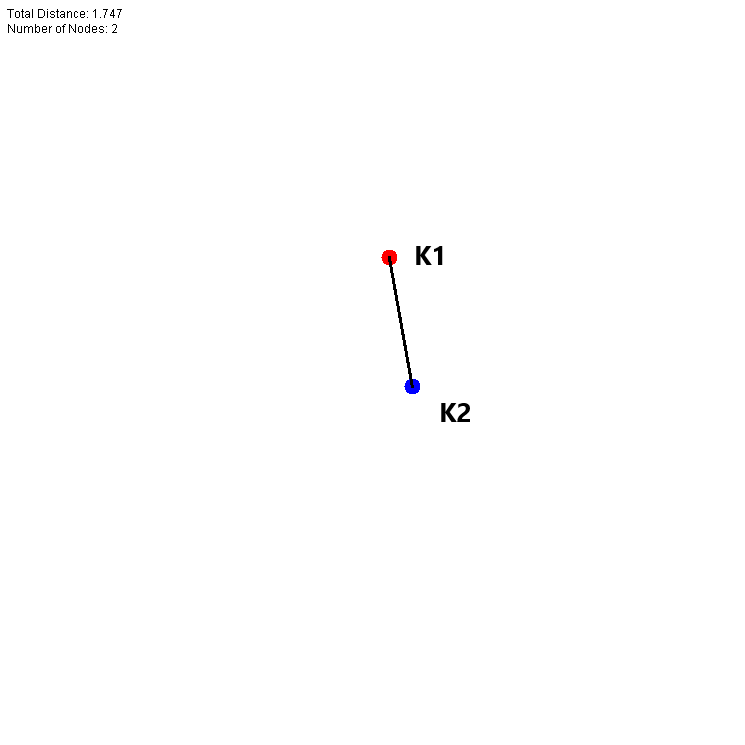
\includegraphics[width=0.35\textwidth]{./Bilder/insertFirst/insert_first_BAD_ex_1.PNG}
        }
        \hfil
        \subfloat[$m = 3$\label{subfig:insert-first-BAD-m3}]{%
        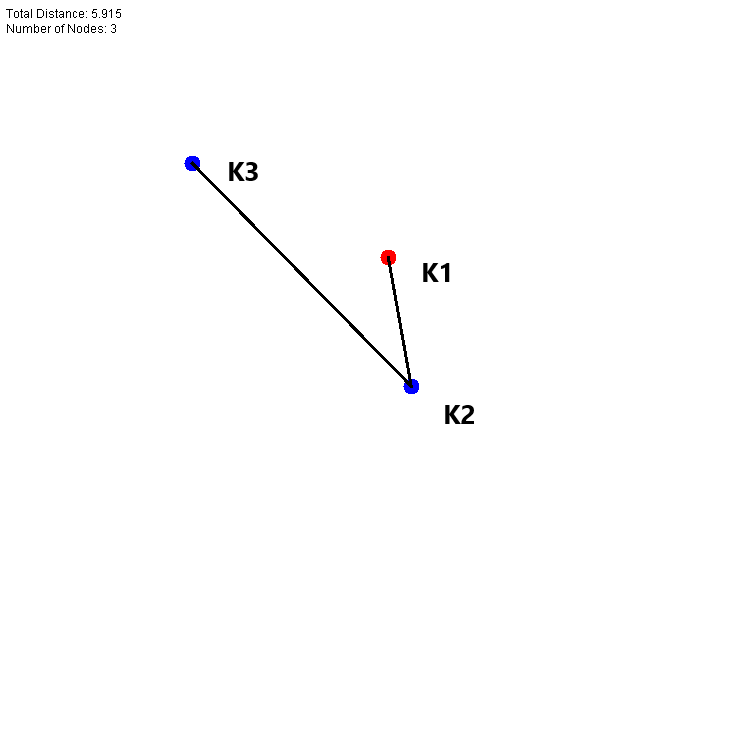
\includegraphics[width=0.35\textwidth]{./Bilder/insertFirst/insert_first_BAD_ex_2.PNG}
        }\\
%     \end{center}
% \end{figure}
% \begin{figure}\ContinuedFloat
%     \begin{center}
        \subfloat[$m = 4$\label{subfig:insert-first-BAD-m4}]{%
        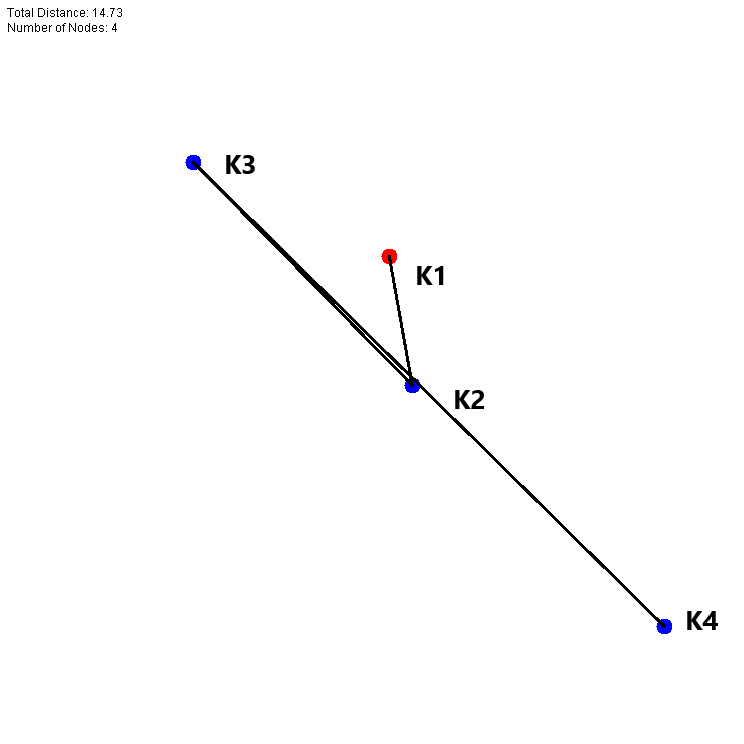
\includegraphics[width=0.35\textwidth]{./Bilder/insertFirst/insert_first_BAD_ex_3.PNG}
        }
        \hfil
        \subfloat[$m = 5$\label{subfig:insert-first-BAD-m5}]{%
        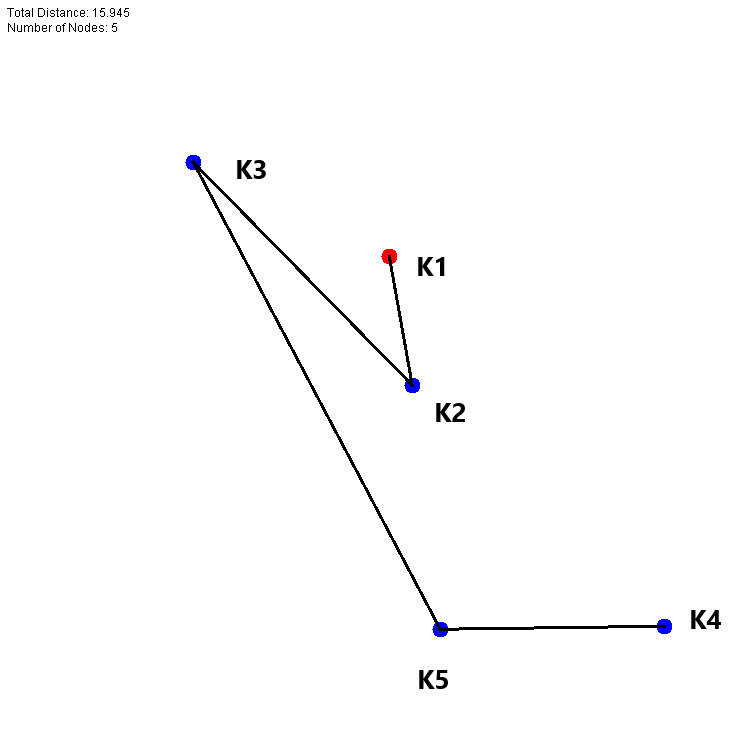
\includegraphics[width=0.35\textwidth]{./Bilder/insertFirst/insert_first_BAD_ex_4.PNG}
        }
        \caption{Insert-First führt zu schlechtem Ergebnis}
        \label{fig:insert-first-bad}
    \end{center}
\end{figure}

% TODO: Alle Schritte/Bilder in den Anhang
Auf \vref{subfig:insert-first-BAD-m4} lässt sich erkennen, dass das Einfügen des vierten Knoten $K_4$ nicht optimal geschieht. 
Besser für $m = 4$ wäre hier der Pfad 
% \begin{addmargin}[1em]{2em}
    $$P=K_1, K_3, K_2, K_4$$
    % \end{addmargin}
Dieser wird allerdings nicht durch das Insert-First-Verfahren gebildet, da dies eine Änderung des bereits erzeugten Graphen in \vref{subfig:insert-first-BAD-m3} erfordern würde. 
Dies ist jedoch nicht möglich, da $K_4$ nur zwischen bereits im Pfad des Graphen vorhandenen Knoten eingefügt werden kann, sodass der schlussendlich generierte Graph eine Gesamtlänge von 15,945 \ac{LE} hat.
Hier lässt sich auch das grundlegende Problem des Algorithmus erkennen: Das Erstellen einer Route ohne vorherige Betrachtung der Gesamtheit der Knoten. 
Einzelne Teilschritte des Graphen können gut erzeugt werden, wie beispielsweise im Schritt von \vref{subfig:insert-first-BAD-m2} zu \vref{subfig:insert-first-BAD-m3}. 
Andere hingegen, wie vorher erwähnt, nicht. 
Grund hierfür ist die alleinige Betrachtung des Knotens $K_i$. 
Spezifischer bedeutet das, dass das frühe Einfügen von Knoten in den Pfad eines Graphen später zu Komplikationen führen kann, da es objektiv besser gewesen wäre einen anderen Knoten früher einzufügen.
Am konkreten Beispiel führt die generierte Reihenfolge von 
% \begin{addmargin}[1em]{2em}
    $$P=K_1, K_2, K_3$$
    % \end{addmargin}
in \vref{subfig:insert-first-BAD-m3} dazu, dass $K_4$ nur unter einen vergleichsweise großen Gesamtdistanzzuwachs in den Graphen eingefügt werden kann. 
\\\\
Konträr zu diesem schlechten Beispiel ist der Insert-First-Algorithmus auch in der Lage gute bis optimale Ergebnisse zu generieren. 

\begin{figure}[H]
    \begin{center}
        \subfloat[$m = 2$\label{subfig:insert-first-GOOD-m2}]{%
        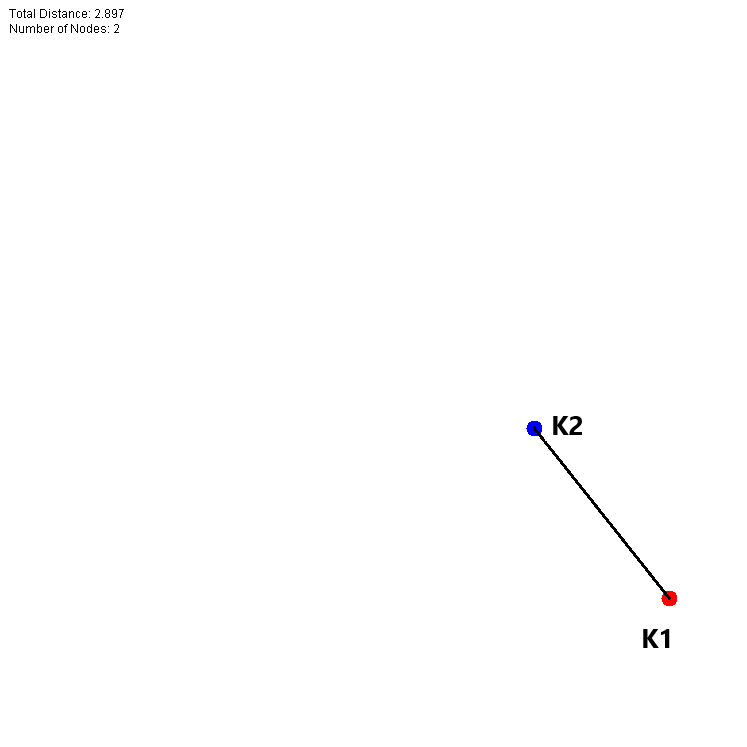
\includegraphics[width=0.35\textwidth]{./Bilder/insertFirst/insert_first_ex_1.PNG}
        }
        \hfil
        \subfloat[$m = 3$\label{subfig:insert-first-GOOD-m3}]{%
        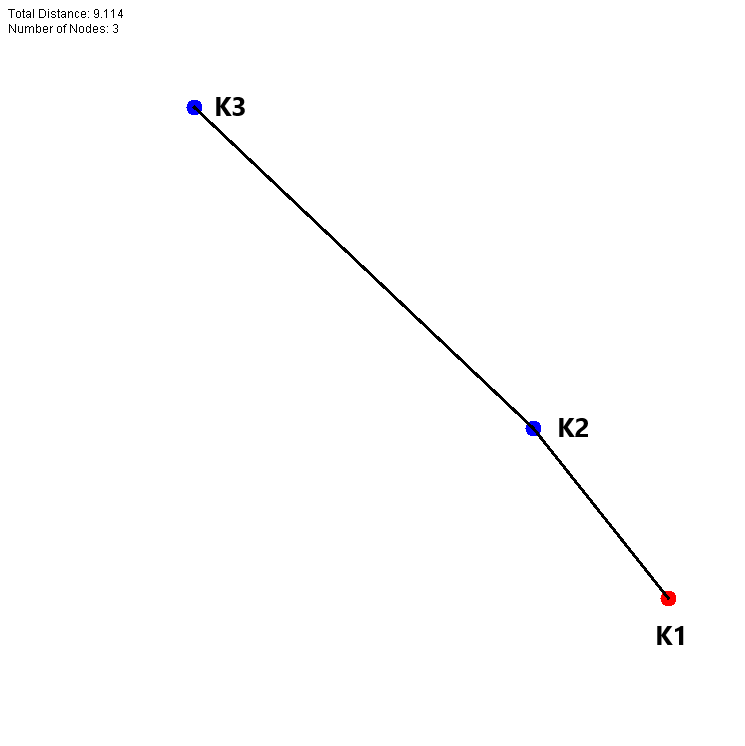
\includegraphics[width=0.35\textwidth]{./Bilder/insertFirst/insert_first_ex_2.PNG}
        }\\
%     \end{center}
% \end{figure}
% \begin{figure}
%     \begin{center}\ContinuedFloat
        \subfloat[$m = 4$\label{subfig:insert-first-GOOD-m4}]{%
        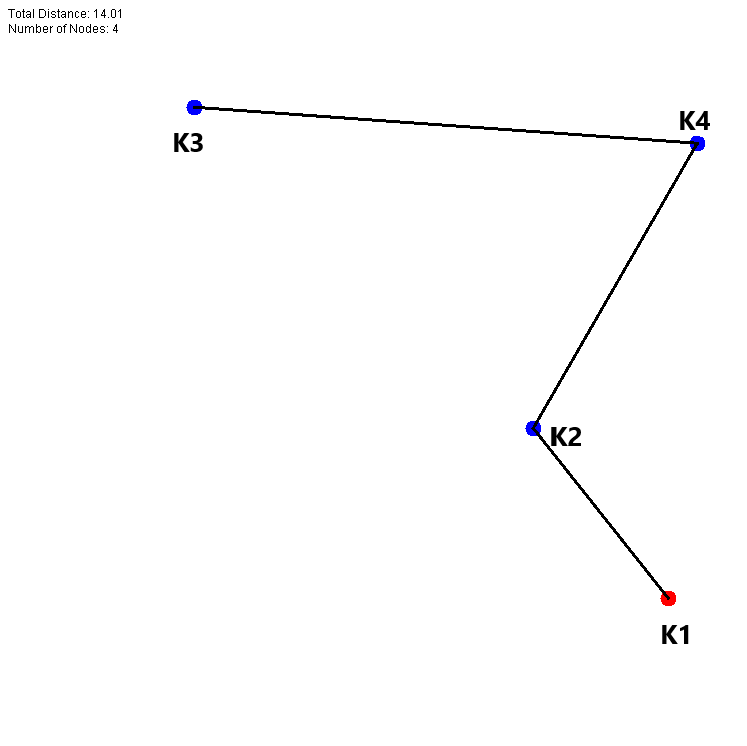
\includegraphics[width=0.35\textwidth]{./Bilder/insertFirst/insert_first_ex_3.PNG}
        }
        \hfil
        \subfloat[$m = 5$\label{subfig:insert-first-GOOD-m5}]{%
        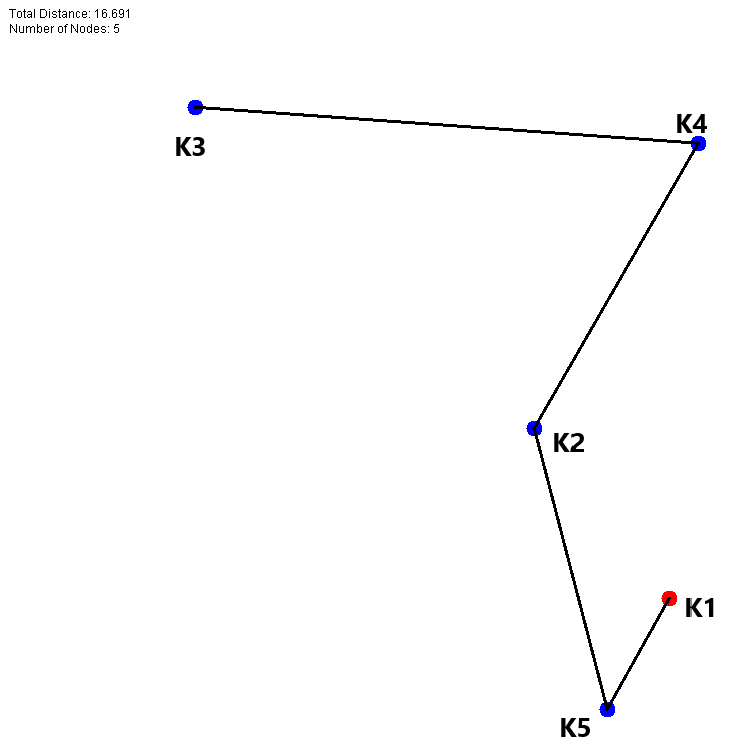
\includegraphics[width=0.35\textwidth]{./Bilder/insertFirst/insert_first_ex_4.PNG}
        }
        \caption{Insert-First führt zu guten Ergebnis}
        \label{fig:insert-first-good}
    \end{center}
\end{figure}
% TODO: Alle Schritte/Bilder in den Anhang

Am Beispiel in \vref{fig:insert-first-good} lässt sich erkennen, wie der Insert-First-Algorithmus einen optimalen Pfad mit den gegebenen Knoten generiert. 
Gerade im Schritt von \vref{subfig:insert-first-GOOD-m4} zu \vref{subfig:insert-first-GOOD-m5} ist ein funktionierendes und korrektes Einfügen des Knotens in den Graphen zu sehen, bei dem der Anstieg der Gesamtdistanz der Route sehr gering gehalten wird. 
Hier wird der aktuelle Knoten mit geringem Zuwachs der schlussendlichen Gesamtdistanz in den Graphen eingefügt, sodass die Gesamtdistanz zum Ende bei 16,691 \ac{LE} liegt.
Die scheint zwar höher als das vorherige schlechte beispiel, das liegt aber an den Positionen der einzelnen Knoten.
\\\\
Für die Bewertung des Algorithmus müssen also beide Seiten betrachtet werden. 
Zwar ist Insert-First in der Lage eine gute oder auch optimale Route zu erstellen, allerdings beeinflusst die Reihenfolge der Betrachtung der Knoten stark die Qualität des Endergebnisses.



\section{Insert-Furthest-Verfahren} \label{sec:insert-furthest-verfahren}
% Was ist das Insert-Furthest-Verfahren?
    % Nodes werden anhand ihrer Entfernung zur vorherigen Node in den Graphen eingefügt
    % Die am weitest entfernten werden zuerst eingefügt
% Was ist das Insert-Furthest-Verfahren
    % Zu Beginn wird wieder die Erste Node in den Pfad eingefügt, um von ihr ausgehend den restlichen Pfad zu bilden
    % anders als bei Insert First muss bzw. kann hier aber nicht auch die zweite Node eingefügt werden, da diese erst noch ermittelt werden muss
    % Spezifische Auswahl der nächsten einzufügenden Node
    % Die als nächstes eingefügt Node ist immer die, die am weitesten von der zuletzt eingefügten Node entfernt ist 
    % Allerdings muss hier vorher die Bedingung geprüft werden, ob die am weitesten Entfernte node nicht schon im Pfad ist
    % Die am weistesten Entfernte Node wird dann genau wie bei Min Dist ist den bereits existierenden Pfad an der besten verfügbaren Stelle eingefügt
    % Ermittlung der Besten Stelle, in die Node Y eingefügt werden: 
        % Es wird durch alle bereits im Graphen vorhandenen Nodes iteriert
        % Die Node der momentanen Iteration X2, ihr Vorgänger X1
        % Die Distanz berechnet sich aus der Entfernung von X1 zu Y addiert mit der Entfernung von Y zu X2
        % Es wird davon ausgegangen, dass X1 immer definiert, also teil des bereits bestehenden Graphen ist, ist 
        % X2 muss nicht zwangweise definiert sein, kann also auch null sein
        % Ist dies der fall wird für die Distanz zwischen Y und X2 0 angenommen
\subsection{Funktionsweise} \label{sec:insert-furthest-funkt}
Aufbauend auf den Erkenntnissen des Insert-First-Verfahrens können experimentell einige Verbesserungsideen abgeleitet und ihre Auswirkungen auf die Erzeugung eines Pfads betrachtet werden.
Bei Betrachtung der Ergebnisse des Insert-First-Algorithmus wurde festgestellt, dass eine große Schwäche des Algorithmus die Reihenfolge der Betrachtung der Knoten sein kann.
Ein möglicher Ansatz, dieser in \vref{sec:inserst-first-erg} beschriebenen Schwäche entgegenzuwirken, ist die Einführung eines Kriteriums für eben diese Reihenfolge der Betrachtung der Knoten.
Eine mögliche Umsetzung eines solchen Kriteriums ist das Insert-Furthest-Verfahren. 
Hier wird der als nächstes einzufügende Knoten ($k_i$) durch seine Distanz zum Vorgänger ($k_{i-1}$) bestimmt.


% \subsection{Funktionsweise}

Ähnlich dem Insert-First-Verfahren wird auch hier ein Graph mit einer Liste von Knoten und einem zu Beginn leerem Pfad erzeugt.
Auch hier wird wieder der erste Knoten der Liste $k_1$ als initialer Knoten $p_1$ des Pfades $P$ gesetzt.
Der nächste zu betrachtende Knoten ist nun aber nicht $k_2$, sondern wird durch die Distanz zu $k_1$ bestimmt.
Ausgewählt wird der Knoten, der am weitesten von $k_1$, bzw. allgemein am weistesten von $k_{i-1}$, entfernt ist und nicht bereits Teil des Pfads ist.
Dieser Knoten wird nun auf die gleiche Weise wie die Knoten beim Insert-First-Verfahren in den Pfad des Graphen eingefügt; die Stelle mit der geringsten Distanzerhöhung für den Graphen wird ermittelt und $k_i$ an dieser Stelle nach dem im Algorithmus \vref{alg:merge-node-into-path} beschriebenen Verfahren eingefügt.\\
Der Gedanke hinter der dieser Veränderung ist der Versuch Knoten mit größerer Vorraussicht als im Insert-First-Verfahren in den Pfad einzufügen.
Ziel ist es mit den ersten paar Knoten einen Pfad zu generieren, der einen großen Teil der Fläche überspannt, auf der sich Knoten befinden.
Das kann insofern zu einem besserem Ergebnis führen, dass die ersten Knoten zwar unter einer -- relativ zur schlussendlichen Gesamtlänge des Graphen -- hohen Distanzerhöhung eingefügt werden, die nachfolgenden Knoten aber durch geringe Umwege des bestehenden Pfads in den Graphen eingebunden werden können.
Auf diese Weise sollen Komplikationen beim Einfügen der letzten Knoten verhindert werden und so suboptimale Graphen wie in \vref{fig:insert-first-bad} umgangen werden. Algorithmus \vref{alg:insert-furthest} zeigt eine beispielhafte Umsetzung des Algorithmus in Pseudocode.

\begin{algorithm}[H]
    \caption{Insert-Furthest-Algorithmus}
    \label{alg:insert-furthest}
    \begin{algorithmic}[1]
        \Require Graph $G$, Pfad $P$ 
        \Require $G=(K,E),K= k_1,k_2,\ldots,k_n$, $n > 2$ 
        % \Require $P=p_1,\cdots,p_m$, $\forall p = k_G$
        \State $p_1 \gets k_1$
        \Comment Setzen des ersten Knoten
        % Find furthest
        \State $i \gets -1$
        \State $d_i \gets -1$

        \For{$a \gets 1$, $a \leq n$, $a \gets a + 1$}
            % Main Loop
            % find Furthest from last
            \State $j_F \gets -1$
            \State $d_F \gets -1$

            \For{$b \gets 2$, $b \leq n$, $b \gets b + 1$}
                \Comment Finde $k_b$ mit der höchsten Distanz zu $p_m$
                \State $d_C \gets \omega$($k_b$, $p_m$)
                \Comment Distanz zwischen $k_b$ und letztem Knoten $p_m$
                \If{$k_b \not \in P$ \textbf{and} ($j_F = -1$ \textbf(or) $d_C > d_F$)}
                    \State $d_F \gets d_C$
                    \State $j_F \gets b$
                \EndIf
            \EndFor

            \State $i_S \gets -1$
            \State $d_S \gets -1$

            \For{$b \gets 2$, $b < m$, $b \gets b + 1$}
                \State $d_C \gets$ \textsc{mergeAt}($P$, $b$, $k_{j_F}$) \textsc{distance}
                \Comment Gesamtlänge des entstehenden Pfads
                \If{$i_S = -1$ \textbf{or} $d_C < d_S$}
                    \State $i_S \gets b$
                    \State $d_S \gets d_C$
                \EndIf
            \EndFor
            \State $P \gets$ \textsc{mergeAt}($P$, $k_{j_F}$, $i_S$)
            \Comment Siehe Alg. \vref{alg:merge-node-into-path}
        \EndFor \\
        \Return new Graph($P$)
    \end{algorithmic}
\end{algorithm}

\subsection{Zeitkomplexität}
Der Insert-Furthest-Algorithmus fügt verglichen mit dem Insert-First-Algorithmus ein Auswahlkriterium hinzu.
Dieses Kriterium drückt sich im Pseudocode im Algorithmus \vref{alg:insert-furthest} durch eine zusätzliche Schleife in Zeile vier aus.
Um nun die Zeitkomplexität zu ermitteln, reicht es die Laufzeit dieser Schleife, $n^2$, auf die in \vref{sec:time-comp-first} berechnete zu addieren, wodurch sich 
$$f(n) = \frac{n^2+n}{2}+n^2 -1$$
und dadurch auch hier eine Komplexität von
$$f(n) = O(n^2)$$
ergibt.
Damit skaliert dieser Algorithmus bei sich verändernder Eingabe in etwa genauso wie Insert-First.

\subsection{Ergebnis und Schwächen}
Testet man des Insert-Furthest-Verfahren anhand der Knoten des Beispiels \vref{fig:insert-first-bad} wird sichtbar, dass der Algorithmus tatsächlich in der Lage ist einen besseren Pfad zu generieren als das Insert-First-Verfahren.

\begin{figure}[H]
    \begin{center}
        % \subfloat[$m = 2$\label{subfig:insert-first-BAD-m2}]{%
        % 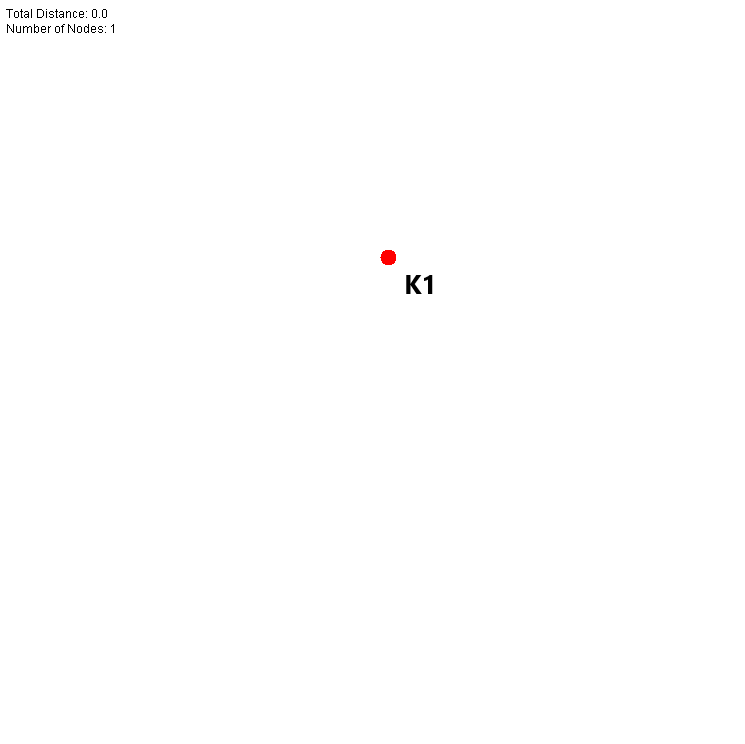
\includegraphics[width=0.35\textwidth]{./Bilder/insertFurthest/insert_furthest_ex_1.PNG}
        % }
        % \hfil
        \subfloat[$m = 2$\label{subfig:insert-furthest-GOOD-m2}]{%
        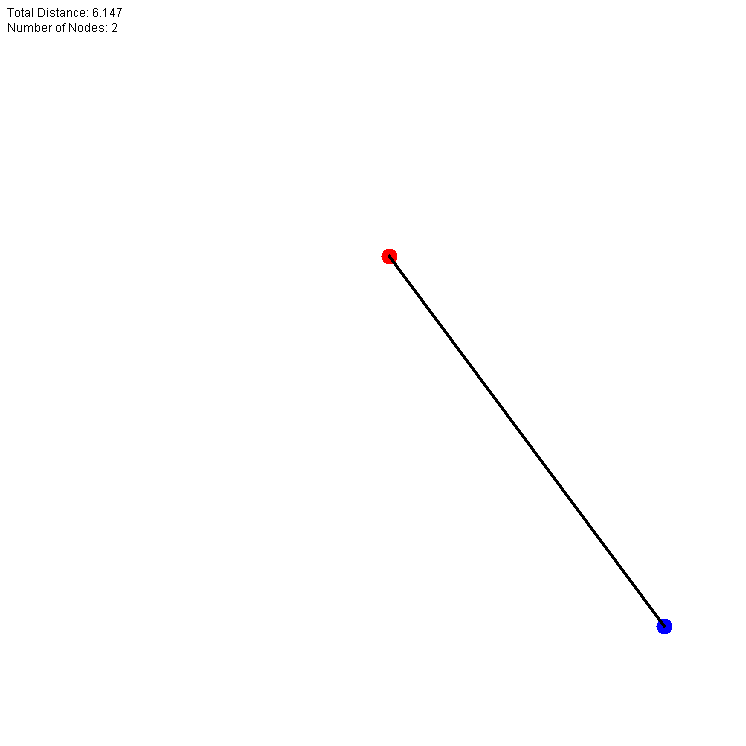
\includegraphics[width=0.35\textwidth]{./Bilder/insertFurthest/insert_furthest_ex_2.PNG}
        }
        % \\
        % \subfloat[$m = 4$\label{subfig:insert-first-BAD-m4}]{%
        % 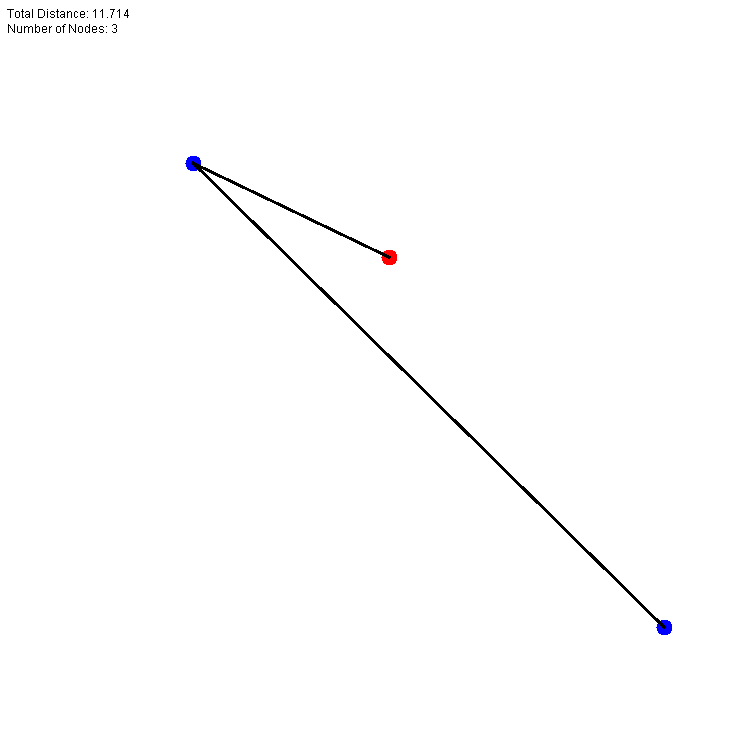
\includegraphics[width=0.35\textwidth]{./Bilder/insertFurthest/insert_furthest_ex_3.PNG}
        % }
        \hfil
        \subfloat[$m = 5$\label{subfig:insert-furthest-GOOD-m5}]{%
        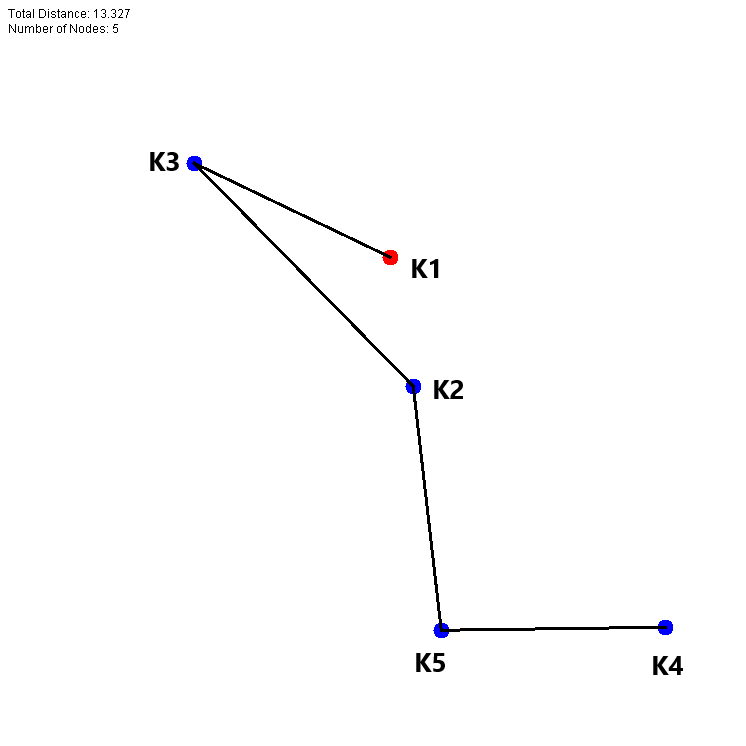
\includegraphics[width=0.35\textwidth]{./Bilder/insertFurthest/insert_furthest_ex_5.PNG}
        }
        \caption{Insert-First führt zu einem gutem Ergebnis}
        \label{fig:insert-furthest-good}
    \end{center}
\end{figure}
Der vollständige Generierungsvorgang befindet sich im Anhang (Abbildung A.3 im Anhang). \\

% TODO: Alle Schritte/Bilder in den Anhang
In \vref{subfig:insert-furthest-GOOD-m2} ist zu erkennen, dass, anstatt wie in \vref{subfig:insert-first-BAD-m2} $k_2$, $k_4$ als erster Knoten eingefügt wird.
Dieses Verhalten ist nach der in \vref{sec:insert-furthest-funkt} definierten Funktionsweise zu erwarten, da $k_4$ der Knoten mit der größten Distanz zu $k_1$ ist und daher als erstes in den Pfad des Graphen eingefügt wird.
Nach der Ausführung aller Schritte des Algorithmus wird der in \vref{subfig:insert-furthest-GOOD-m5} zu sehenden Graphen generiert.
Dieser hat eine Gesamtdistanz von 13,327 \ac{LE} und ist somit im Vergleich mit dem in \vref{fig:insert-first-bad} durch das Insert-First-Verfahren erzeugten Graph 2,618 \ac{LE} oder 16,41\% kürzer.
\\\\
Ebenso wie das Insert-First-Verfahren kann das Insert-Furthest-Verfahren auch Graphen generieren die in ihrer Gesamtdistanz vom Optimum abweichen. Am folgenden Beispiel wird deutlich, dass auch dieser Algorithmus von ähnlichen Schwächen betroffen ist.
\begin{figure}[H]
    \begin{center}
        % \subfloat[$m = 2$\label{subfig:insert-first-BAD-m2}]{%
        % 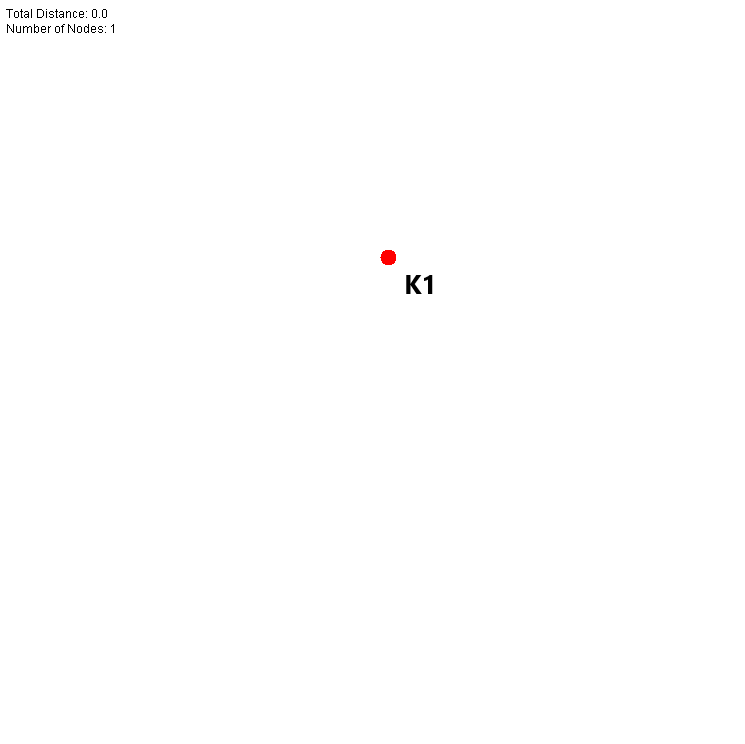
\includegraphics[width=0.35\textwidth]{./Bilder/insertFurthest/insert_furthest_ex_1.PNG}
        % }
        % \hfil
        \subfloat[$m = 4$\label{subfig:insert-furthest-BAD-m2}]{%
        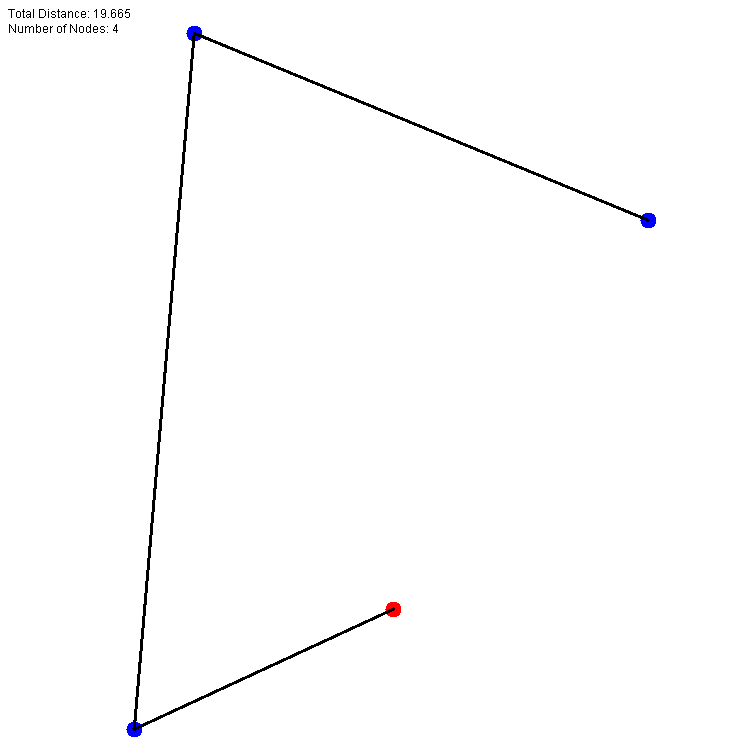
\includegraphics[width=0.35\textwidth]{./Bilder/insertFurthest/insert_furthest_ex_BAD_4.PNG}
        }
        % \\
        % \subfloat[$m = 4$\label{subfig:insert-first-BAD-m4}]{%
        % 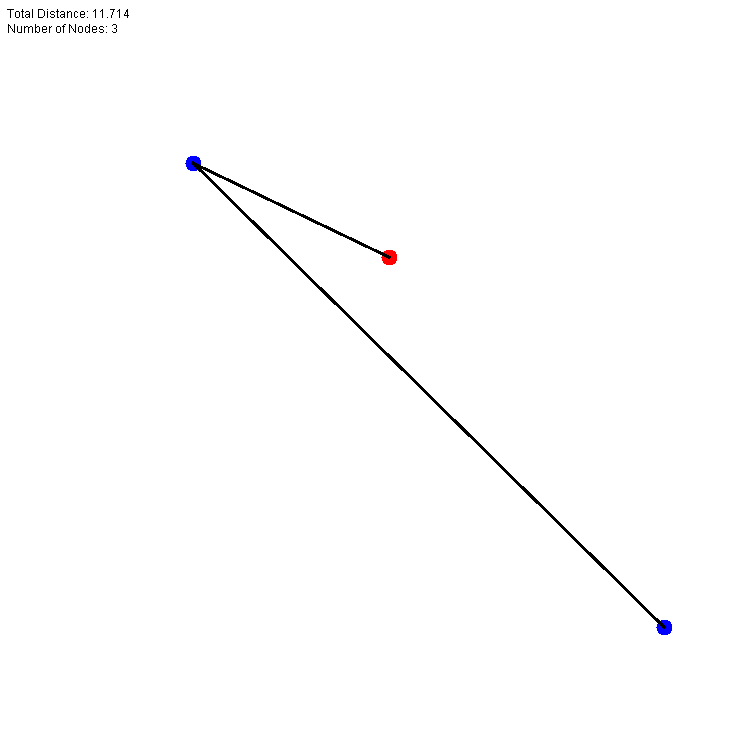
\includegraphics[width=0.35\textwidth]{./Bilder/insertFurthest/insert_furthest_ex_3.PNG}
        % }
        \hfil
        \subfloat[$m = 5$\label{subfig:insert-furthest-BAD-m5}]{%
        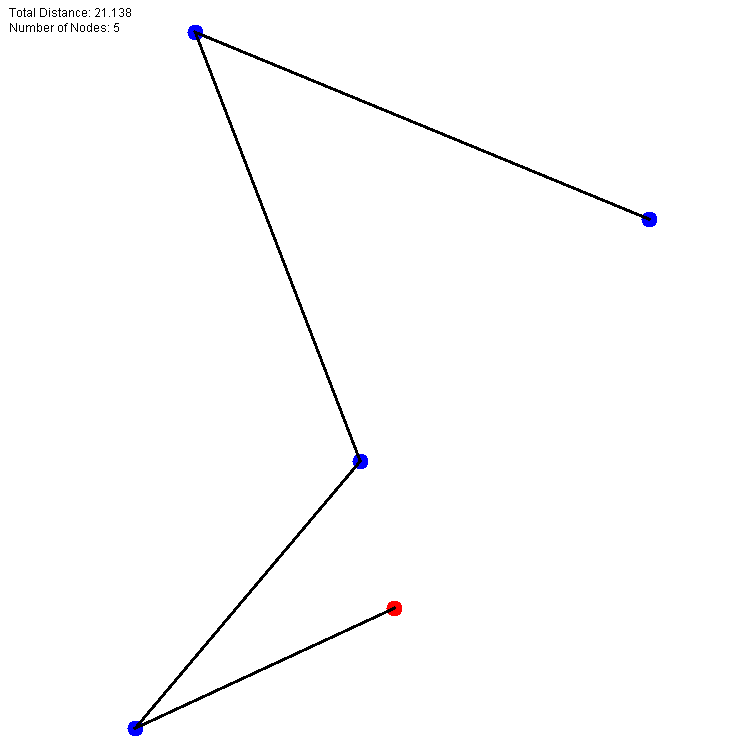
\includegraphics[width=0.35\textwidth]{./Bilder/insertFurthest/insert_furthest_ex_BAD_5.PNG}
        }
        \caption{Insert-First führt zu einem schlechtem Ergebnis}
        \label{fig:insert-furthest-bad}
    \end{center}
\end{figure}
% TODO: Bilder in den Anhang
Der vollständige Generierungsvorgang befindet sich im Anhang (Abbildung A.4 im Anhang). \\
\\\\
Auch hier lässt sich das Problem der Reihenfolge beobachten, welches in \vref{sec:inserst-first-erg} beschrieben wurde.
Durch das Einfügen des letzten Knotens $k_4$ in den Pfad entsteht ein suboptimaler Graph.
Werden die Distanzen zwischen den Knoten $k_4$ und $k_5$ (6,129 \ac{LE}) mit den zwischen $k_5$ und $k_2$ (5,019 \ac{LE}) verglichen, wird schnell ersichtlich, dass eine Verminderung der Distanz durch das Umlegen der Knoten erreicht werden kann.
Verursacht wird diese Abweichung vom Optimum dadurch, dass $k_4$ als letztes in den Graphen eingefügt wird, da der Knoten sich, relativ zu den restlichen Knoten, in der Mitte der Fläche befindet und somit aufgrund seiner geringeren Entfernung zu anderen Knoten vom Algorithmus als letztes betrachtet wird.
Die optimale Route
% \begin{addmargin}[1em]{2em}
$$P = k_1, k_3, k_4, k_2, k_5$$ 
    % \end{addmargin}
 würde es jedoch erfordern, dass $k_4$ früher betrachtet und in den Pfad eingefügt wird.
Der durch den Algorithmus erzeugte Graph hat eine Gesamtlänge von 21,138 \ac{LE}, während durch das Umlegen zum optimalen Graph eine Länge von 20,028 \ac{LE}, also Reduktion der Distanz um 1,11 \ac{LE} oder 5,251\% erreicht werden kann.
\\\\
Das Insert-Furthest-Verfahren verhält sich in einigen Fällen, wie in \vref{fig:insert-furthest-good} gezeigt, besser als das Insert-First-Verfahren, weist aber immer noch eindeutige Schwächen, gerade im Bezug auf die Reihenfolge der Betrachtung der Knoten, auf.
Das Beispiel in \vref{fig:insert-furthest-bad} zeigt deutlich, wie auch hier die Positionierung der Knoten einen negativen Einfluss auf das Endergebnis hat.
\section{Insert-Closest-Verfahren}
    % Was ist das Min-Dist-Verfahren
        % Umgekehrtes Prinzip von Insert Furthest
        % Allerdings wird nun die nächste Node an den Graphen angehängt
    % Wie funktioniert das Min-Dist-Verfahren
        % Zuerst wird die Node in den Graphen eingefügt, welche den niedrigsten Index im Node Array hat (also am Anfang steht)
        % Dann nun wird die Node gesucht, welche am Nächsten an der ersten Node ist
        % Dazu wird einfach durch alle Nodes iteriert, die Entfernungen berechnet und dadurch die Node mit der geringsten Entfernung ermittelt
        % Diese wird dann an den Graphen angehängt, das heißt in die erste leere Stelle eingefügt
    \subsection{Funktionsweise}
Aufbauend auf den durch das Insert-First- und Insert-Furthest-Verfahren gewonnen Erkenntnissen ist es mögliche weitere Variationen der Heuristik zu entwickeln und deren Ergebnisse zu betrachten.
Da sowohl in \vref{sec:insert-first-verfahren} als auch in \vref{sec:insert-furthest-verfahren} festgestellt wurde, dass ein Grund für suboptimal erstellte Routen die Reihenfolge der Betrachtung der Knoten ist, wird für das Insert-Closest-Verfahren eine weitere anderes Kriterium für eben diese Reihenfolge festgelegt.
Wie der Name des Verfahrens schon suggeriert, geschieht hier die Auswahl der Knoten wieder nach ihrer Distanz.


Das Insert-Closest-Verfahren bezeichnet im Grundprinzip die Umkehrung des Insert-Furthest-Prinzips. 
Anstatt des am weitesten entfernten Knotens wird hier der dem aktuellen Knoten nächste betrachtet.
\\
Zu Beginn beschreibt sich der Algorithmus identisch zum Insert-Furthest-Verfahren.
Auch hier wird ein neuer Graph mit einem leerem Pfad \lstinline{path} und einer Liste von Knoten $K_1, \dots ,K_n$ der Länge $n$ erzeugt.
Auch hier wird der erste Knoten $K_1$ als erster Knoten des Pfades festgelegt.
Der als nächstes einzufügende Knoten wird wie beim Insert-Furthest-Verfahren durch seine Distanz zum vorherigen bestimmt.
Für das Insert-Closest-Verfahren wird der dem Vorherigen Knoten nächste Knoten, unter der Bedingung, dass dieser nicht bereits Teil des Graph ist, in den Pfad eingefügt.
Um die beste Stelle zum Einfügen des Knotens zu ermitteln wird das gleiche Verfahren wie bei den beiden vorherigen Algorithmen angewandt; die Stelle, die den geringsten Anstieg für die Gesamtdistanz des Pfads wird ausgewählt.
Auch das Vorgehen beim Einfügen orientiert sich hier an den vorherigen Algorithmen.
Der aktuelle Knoten $K_i$ wird nach dem in \vref{alg:merge-node-into-path} dargestelltem Prinzip an dem vorher festgelegten Index $j$ in den Graph eingefügt.
\\
Der beschriebene Algorithmus befindet sich als Pseudocode in etwas ausführlicher Version unter \ac{Alg.} \vref{alg:insert-furthest}.
\begin{algorithm}
    \caption{Insert-Closest-Algorithmus}
    \label{alg:insert-closest}
    \begin{algorithmic}[1]
        \Require Graph $G$, Pfad $P$
        \Require $G = K_1,K_2,\ldots,K_n$, $n > 2$
        \State $p_1 \gets K_1$
        \Comment Setzen des ersten Knoten
        % Find furthest
        \State $i \gets -1$
        \State $d_i \gets -1$

        \For{$a \gets 1$, $a \leq n$, $a \gets a + 1$}
            % Main Loop
            % find Furthest from last
            \State $j_S \gets -1$
            \State $d_S \gets -1$

            \For{$b \gets 2$, $b \leq n$, $b \gets b + 1$}
                \Comment Finde $K_b$ mit der geringsten Distanz zu $p_m$
                \State $d_C \gets$ \textsc{distance}($K_b$, $p_m$)
                \Comment Distanz zwischen $K_b$ und letztem Knoten $p_m$
                \If{$K_b \not \in P$ \textbf{and} ($j_S = -1$ \textbf(or) $d_C > d_S$)}
                    \State $d_S \gets d_C$
                    \State $j_S \gets b$
                \EndIf
            \EndFor

            \State $i_S \gets -1$
            \State $d_S \gets -1$

            \For{$b \gets 2$, $b < n$, $b \gets b + 1$}
                \State $d_C \gets$ \textsc{mergeAt}($P$, $b$, $K_{j_F}$) \textsc{distance}
                \If{$i_S = -1$ \textbf{or} $d_C < d_S$}
                    \State $i_S \gets b$
                    \State $d_S \gets d_C$
                \EndIf
            \EndFor
            \State $P \gets$ \textsc{mergeAt}($P$, $K_{j_S}$, $i_S$)
            \Comment Siehe Alg. \vref{alg:merge-node-into-path}
        \EndFor \\
        \Return new Graph($P$)
    \end{algorithmic}
\end{algorithm}

\subsection{Zeitkomplexität}
Da es sich beim Insert-Closest-Algorithmus im eine Abwandlung des Insert-Furthest handelt, ist die Struktur beider Algorithmen gleich -- nur eine Bedingung ändert sich.
Daher kann auch für diesen Algorithmus eine Zeitkomplexität von $$O(n) = n^2$$ angenommen werden, womit auch dieser Algorithmus wie Insert-First skaliert.

\subsection{Ergebnis und Schwächen}
Auch die Ergebnisse dieses Algorithmus gestalten sich sehr divers.
Wie bei den beiden anderen Verfahren entstehen hier Graphen, die nahe an die Optimale Route heranreichen oder ihr teilweise auch entsprechen, aber auch solche, die weit von der optimalen Lösung abweichen.
Übergibt man dem Algorithmus beispielsweise die gleichen Knoten wie in Abbildung \vref{fig:insert-first-bad}, einem Szenario, bei dem der Insert-First Algorithmus einen suboptimalen Graph generiert, kommt der Insert-Closest Algorithmus, so wie der Insert-Furthest Algorithmus auch, auf die optimale Route.\\
So wie die anderen Algorithmen stößt aber auch der Insert-Closest Algorithmus bei bestimmten Konstellationen von Knoten an seine Grenzen.

\begin{figure}
    \begin{center}
        \subfloat[$m=4$ \label{subfig:insert-closest-BAD-4}]{
            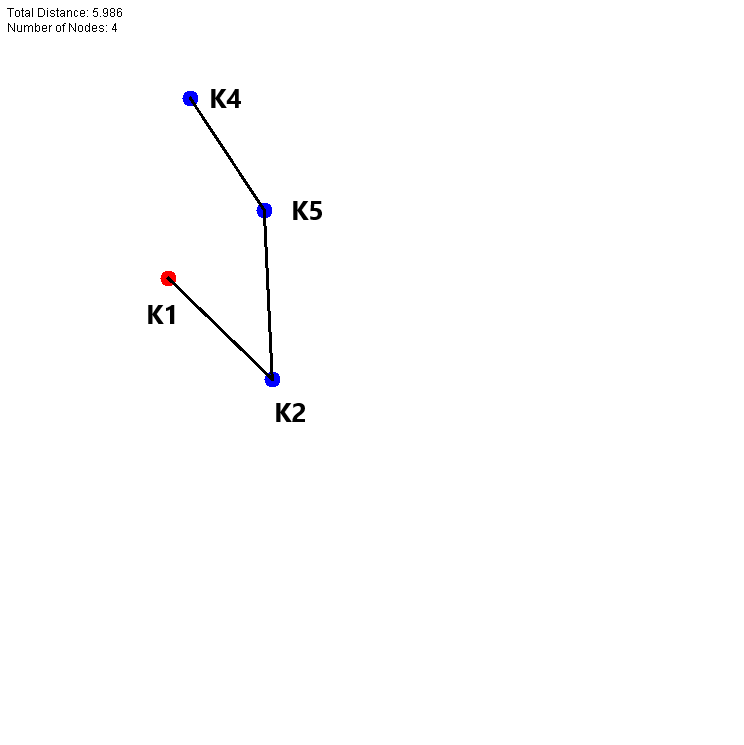
\includegraphics[width=0.35\textwidth]{Bilder/insertClosest/insert_closest_ex_BAD_4.PNG}
        }
        \hfil
        \subfloat[$m=5$ \label{subfig:insert-closest-BAD-5}]{
            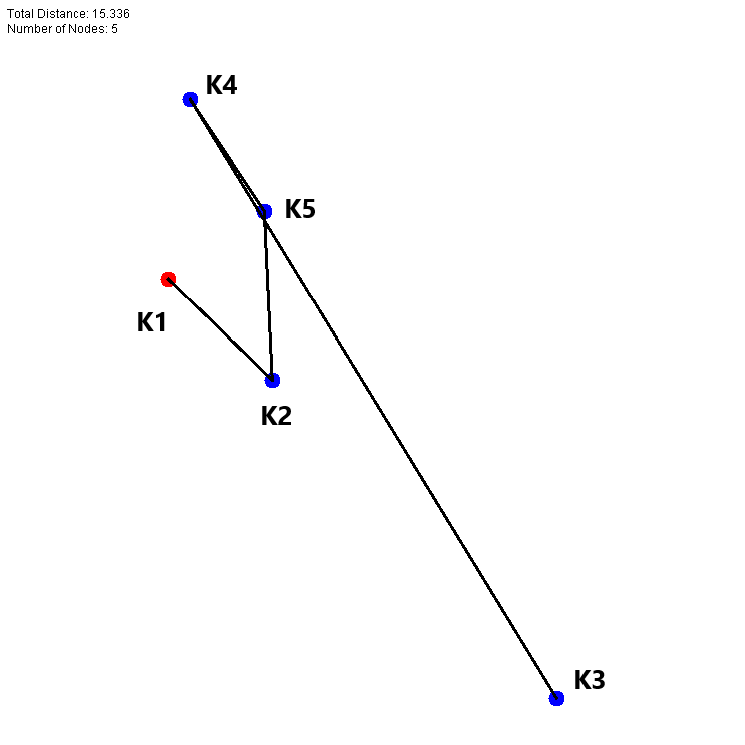
\includegraphics[width=0.35\textwidth]{Bilder/insertClosest/insert_closest_ex_BAD_5.PNG}
        }
        \caption{Der Insert-Closest Algorithmus kommt zu einem schlechten Ergebnis}
        \label{fig:insert-closest-BAD}
    \end{center}
\end{figure}

Wie in Abbildung \vref{fig:insert-closest-BAD} zu sehen ist, plant der Algorithmus einen Pfad, der deutlich erkennbar nicht optimal ist.
Die einzelnen Schritte, die zur Generierung des Graphen führen finden sich im Anhang in der Abbildung \vref{app:fig:insert-closest-BAD-complete}.
Der in \vref{subfig:insert-closest-BAD-5} gezeigt Pfad hat eine Gesamtdistanz von 15,336 \ac{LE}.
Durch das Ändern der Reihenfolge der Knoten zu
% \begin{addmargin}[1em]{2em}
    $$P=K_1, K_4, K_5, K_2, K_3$$ 
% \end{addmargin}
könnte eine Verringerung der Distanz im Vergleich zum vorherigen Resultat um 3,208 \ac{LE}, bzw. 20,918\% erreicht werden.
Auch hier wird der suboptimal geplante Pfad durch die Reihenfolge der Betrachtung der Knoten verursacht.
Im konkreten Beispiel werden die ersten vier Knoten $K_1, K_2, K_4$ und $K_5$ zu einem für sich optimalen Pfad zusammengefügt.
$K_3$ wird aufgrund seiner hohen Distanz zu den übrigen Knoten als letztes in den Pfad eingefügt.
Im gezeigten Beispiel kommt es also genau zu der Umkehrung des Problems, welches beim Insert-Furthest Algorithmus besteht; dort werden Knoten aufgrund ihrer zu niedrigen Distanz teilweise zu spät eingefügt.
Diese Problem hat hier zur Folge, dass $K_3$ als letzter Knoten des Pfads nach dem von ihm am weitesten entfernten Knoten eingefügt wird, was zu einem hohen Zuwachs der Gesamtdistanz führt.
\section{Lösungsverfahren im Vergleich}
% Vergleichen,
Betrachtet man die Graphen, die durch die drei vorgestellten Algorithmen erzeugt werden, so fallen bei allen schnell Schwächen auf, die ihr Ergebnis beeinträchtigen.

\chapter{Verbesserung eines bestehenden Pfads}

\section{Entfernen von Überschneidungen}
\subsection{Beschreibung des Problems}
Wie in Abschnitt \vref{sec:allBet} angedeutet kommt es kommt es bei generierten Graphen zu Überkreuzungen von Teilrouten zwischen jeweils zwei Knoten.
Betrachtet man solche Überkreuzungen im Detail fallen einige Gemeinsamkeiten zwischen ihnen auf.
So ist es beispielsweise immer möglich eine Überkreuzung durch das Verändern der Reihenfolge der Knoten im Pfad aufzulösen und so eine Verringerung in der Gesamtdistanz zu erreichen.

\begin{figure}[h]
    \begin{center}
        \subfloat[Graph mit einer Überkreuzung\label{subfig:graph-with-crossover-and-rect}]{
            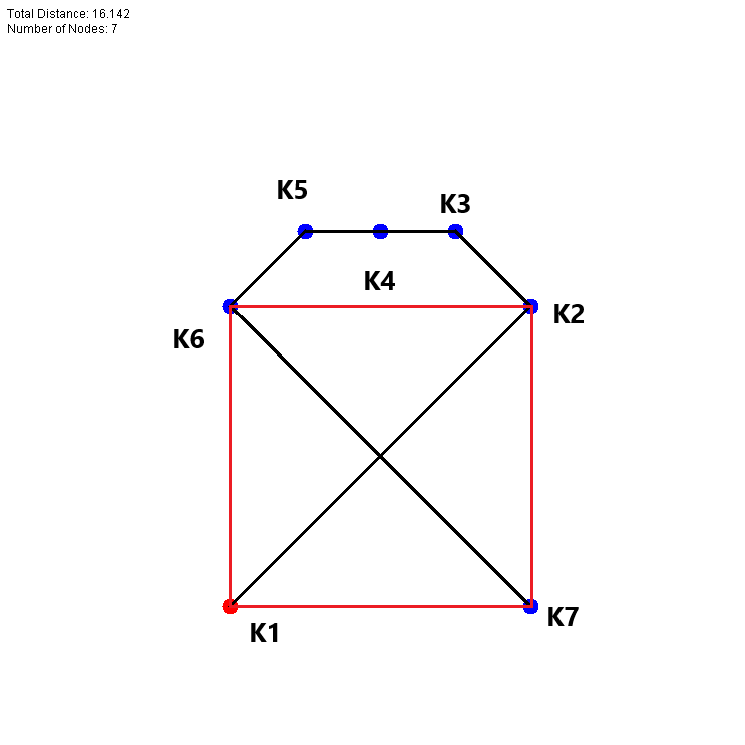
\includegraphics[width=0.35\textwidth]{Bilder/crossover/7_nodes_with_crossover.PNG}
        }
        \hfil
        \subfloat[Aufgelöste Überkreuzung\label{subfig:graph-without-crossover}]{
            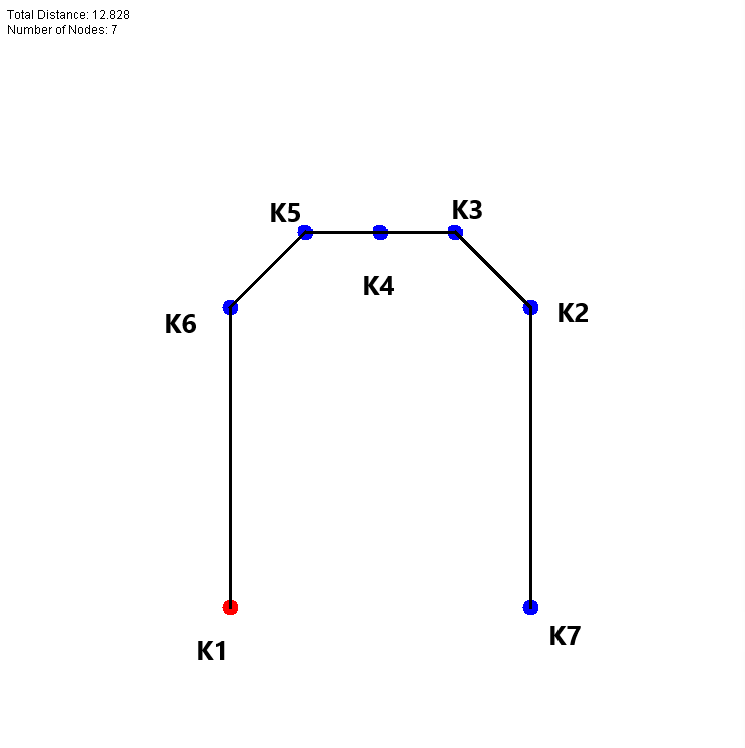
\includegraphics[width=0.35\textwidth]{Bilder/crossover/7_nodes_without_crossover.PNG}
        }
        \caption{Graph mit und ohne Überkreuzung (Das rote Rechteck in Abbildung a) dient späteren Illustrationszwecken)}\label{fig:graph-with-and-without-crossover}
    \end{center}
\end{figure}

Anhand dieses Beispiels wird nun das Entstehen, Erkennen und Auflösen von Überkreuzungen erläutert.

% Allgemein
Eine Überkreuzung repräsentiert das Auftreten eines Schnittpunkts von zwei Kanten eines Graphen in einem für den Graphen relevanten Bereich.
Ein Schnittpunkt von zwei Kanten bedeutet hier, dass keine der vier Knoten gleich sein dürfen.
Besteht eine Überkreuzung also aus den Knotenpaaren $A$ und $B$ mit $A=k_{A_1},k_{A_2}$ und $B=k_{B_1},k_{B_2}$, dann muss gelten $k_{A_1} \neq k_{A_2} \neq k_{B_1} \neq k_{B_2}$.
Ist diese Bedingung nicht erfüllt, kann es keine Überkreuzung geben.
Sind nur drei der vier benötigten Knoten einzigartig kann es nicht zu einer Überkreuzung kommen, da dies einen zusammenhängenden Streckenabschnitt der Form $k_1, k_2, k_3$ darstellen würde.

\subsection{Erkennen von Überkreuzungen} \label{sec:erkennen-von-ueberkreuzungen}
Um Überkreuzungen erkennen zu können, ist die Bedingung \enquote{in einem für den Graphen relevanten Bereich} wichtig.
Betrachtet man zwei zufällig ausgewählte Kanten als unendliche Linien, stellt man sie also in der zweidimensionalen Ebene als lineare Funktion, mit einer Steigung und einem Schnittpunkt mit der Ordinate, dar, dann schneiden sich alle diese Funktionen an irgendeinem Punkt, es sei denn sie sind parallel zueinander.
Um zu überprüfen, ob eine Überkreuzung im für die Generierung eines Graphen relevanten Bereich ist, wird zuerst der Schnittpunkt der beiden Kanten berechnet.
Dazu wird aus zwei Knoten einer Kante eine lineare Funktion der Form $f(x) =mx+n$ simuliert, wobei $m=\frac{\Delta y}{\Delta x}$ und $n=y - mx$.
Sind die Knoten der beiden Kanten nun $A_1,A_2$ und $B_1,B_2$, dann ergibt sich für die Berechnung der Schnittstelle unter der Bedingung, dass $m_A \neq m_B$:
\begin{equation}
    \label{eq:calculation-xs}
    % x_S = (y_{B_1} - (x_{B_1}\cdot \frac{(y_{A_2} - y_{A_1})}{(x_{A_2} - xy_{A_1})}))
    x_S = \frac{(y_{B_1} - \frac{y_{B_2} - y_{B_1}}{x_{B_2} - x_{B_1}}\cdot x_{B_1}) - (y_{A_1} - \frac{y_{A_2} - y_{A_1}}{x_{A_2} - x_{A_1}}\cdot x_{A_1})}{(\frac{y_{A_2} - y_{A_1}}{x_{A_2} - x_{A_1}}) - (\frac{y_{B_2} - y_{B_1}}{x_{B_2} - x_{B_1}})} 
\end{equation}
\begin{equation}
    \label{eq:calculation-ys}
    y_S = \frac{y_{A_2} - y_{A_1}}{x_{A_2} - x_{A_1}}\cdot x_S + (y_{A_1} - \frac{y_{A_2} - y_{A_1}}{x_{A_2} - x_{A_1}}\cdot x_{A_1})
\end{equation}
Mit $x_S$ und $y_S$ lässt sich der Schnittpunkt $S(x_S|y_S)$ konstruieren.
\\\\
Mit Hilfe des Punkts $S$ gilt es nun zu überprüfen, ob sich dieser im relevanten Bereich befindet.
Um dies zu bestimmen wird um die Knoten beider Kanten jeweils ein Rechteck simuliert, wie es beispielhaft in Abbildung \vref{subfig:graph-with-crossover-and-rect} eingezeichnet ist.
Eine Überkreuzung ist genau dann für den Algorithmus relevant, wenn sie in den Rechtecken beider Kanten liegt.
Um dies zu überprüfen wird der in Algorithmus \vref{alg:check-point-in-rect} beschriebene Algorithmus verwandt.
An dieser Stelle sei angemerkt, dass das Problem der Überkreuzungserkennung auch mit Hilfe von Vektorenskalierung lösbar ist.
Ein solches Verfahren wird jedoch in dieser Arbeit nicht ausgearbeitet.


\subsection{Auflösen von Überkreuzungen}

Um einen Algorithmus zur Auflösung von Überkreuzungen entwickeln zu können, ist es wichtig die Knoten um eine Überkreuzung herum vor und nach deren Auflösung zu betrachten.
Dazu kann als Beispiel wieder Abbildung \vref{fig:graph-with-and-without-crossover} dienen.
Die Reihenfolge der Knoten in Abbildung \vref{subfig:graph-with-crossover-and-rect} ist $$P_{alt} = k_1, k_2, k_3, k_4, k_5, k_6, k_7$$
Die Reihenfolge der Knoten nach dem Auflösen der Überkreuzung in Abbildung \vref{subfig:graph-without-crossover} ist $$P_{neu} = k_1, k_6, k_5, k_4, k_3, k_2, k_7$$
In diesem Beispiel seien die betroffenen Kanten $A$ und $B$ mit den Knoten $k_{A_1} = k_1$, $k_{A_2} = k_2$ und $k_{B_1} = k_6$, $k_{B_2} = k_7$.
Die hier interessanten Knoten sind $k_2$ bis $k_6$, da sich deren Reihenfolge umkehrt.
Daraus kann gefolgert werden, dass das Auflösen einer Überkreuzung das Umkehren der betroffenen Knoten in der Mitte bedeutet.
Die betroffenen Knoten bestimmen sich durch die Kanten $A$ und $B$ -- der erste umzukehrende Knoten ist immer $k_{A_2}$, während der letzte $k_{B_1}$ ist.
Dies trifft allerdings nur unter der Bedingung zu, dass $A$ im Graph vor $B$ liegt.
% Ist dies nicht der Fall müssen $A$ und $B$ getauscht werden, sodass 
Ist dies nicht der Fall kehren sich die Rollen der Knoten um und $k_{B_1}$ ist der erste, während $k_{A_2}$ der letzte umzukehrende Knoten ist.
Ein Algorithmus, der auf einem Pfad mit Überkreuzung und bekannten $A$ und $B$ eben dieses Tauschen ausführt, findet sich unter Algorithmus 11 im Anhang. %\vref{alg:swap-nodes-inbetween}.
\\\\
% Ein vollständiger Algorithmus, der die aufgeführten Methodiken anwendet um Überkreuzungen zu erkennen und aufzulösen könnte beispielhaft
Ein vollständiger Algorithmus, der die aufgeführten Methodiken anwenden soll, um Überkreuzungen zu erkennen und aufzulösen, muss also alle Kanten gegeneinander prüfen.
Eine Umsetzung eines solchen Algorithmus findet sich unter Algorithmus \vref{alg:handle-crossover}.
\begin{algorithm}
    \caption{Erkennen und Auflösen von Überkreuzungen auf einem Pfad}
    \label{alg:handle-crossover}
    \begin{algorithmic}[1]
        \Require Pfad $P$
        \Require $P=p_1,p_2\cdots,p_n$, $n \geq 4$, $\forall p \in G$
        
        \For{$a \gets 2$, $a \leq n$, $a \gets a + 1$}
            \For{$b \gets b$, $b \leq n$, $b \gets b + 1$}
                \If{\textbf{not} ($p_a \neq p_{b} \textrm{\textbf{ and }} p_a \neq p_{b-1} \textrm{\textbf{ and }} p_{a-1} \neq p_b \textrm{\textbf{ and }} p_{a-1} \neq p_{b-1}$}
                    \State \textsc{continue}
                \EndIf
                \State $x_S \gets $ nach \vref{eq:calculation-xs}
                \Comment $p_a$ und $p_{a-1}$ entsprechen $A_1$ und $A_2$ 
                \State $y_S \gets $ nach \vref{eq:calculation-ys}
                \Comment $p_b$ und $p_{b-1}$ entsprechen $B_1$ und $B_2$ 
                \If{\textsc{check}($p_a,p_{a-1},S(x_S|y_S)$) \textbf{and} \textsc{check}($p_b,p_{b-1},S(x_S|y_S)$)} 
                % \Comment \textsc{check} repräsentiert dabei Algorithmus 9 im Anhang
                    \State $P \gets $ \textsc{resolve}($P$, $p_a$, $p_{b-1}$)
                %     \Comment Auflösen der Überkreuzung mit Algorithmus 11 im Anhang % \vref{alg:swap-nodes-inbetween}
                \EndIf
            \EndFor
        \EndFor
    \end{algorithmic}
\end{algorithm}

Wird das Entfernen von Überkreuzungen nach diesem Prinzip implementiert, gilt es auch hier wieder die Implikationen einer solchen Implementierung zu betrachten.
Aufgrund der geschachtelten Iterationen über die Kanten des Graphs lässt sich eine Zeitkomplexität von $$f(n) = O(n^2)$$ ermitteln, womit der Algorithmus im Rahmen der polynomialen Zeitkomplexitätsklasse liegt. 
Dies bedeutet, dass die Laufzeit des Algorithmus, wie auch schon bei den vorher vorgestellten Algorithmen, proportional zum Quadrat seiner Eingabemenge wächst.
Als Eingabemenge können hier Knoten bzw. Kanten eines Graphen behandelt werden, wobei $n$ die Menge der Knoten repräsentiert.
\\
Ein Algorithmus, der Überkreuzungen aus einem Graph entfernt, arbeitet also mit einer ähnlichen Laufzeit wie die Heuristiken, die den Graph vorher erzeugen.
\\\\
Weiterhin ist es möglich, dass durch das Auflösen einer Überkreuzung eine weitere, neue entsteht.
Geschieht dies unter der Bedingung, dass in den restlichen Iterationen über die Kanten diese Überkreuzung nicht mehr erkannt wird, beispielsweise, wenn dies in der letzten Iteration passiert, dann wird die Überkreuzung nicht vom Algorithmus aufgelöst.
Eine Möglichkeit dies zu umgehen ist durch das rekursive Aufrufen des Algorithmus, damit mehrmals auf Überkreuzungen überprüft wird.
Allerdings besteht hier Bedarf eine solche Implementierung genauer zu untersuchen, was in dieser Arbeit nicht behandelt wird.


\section{Nachbesserung eines Pfads}
\subsection{Darstellung des Grundproblems}
Neben den im vorherigen Abschnitt beschriebenen Überkreuzungen kommt es bei den generierten Graphen auch zu solchen, die durch ein einfaches Umlegen der Route verbessert werden können.

\begin{figure}[h]
    \begin{center}
    
    \subfloat[Verbesserungsfähiger Graph \label{subfig:after-control-ex1-1}]{
        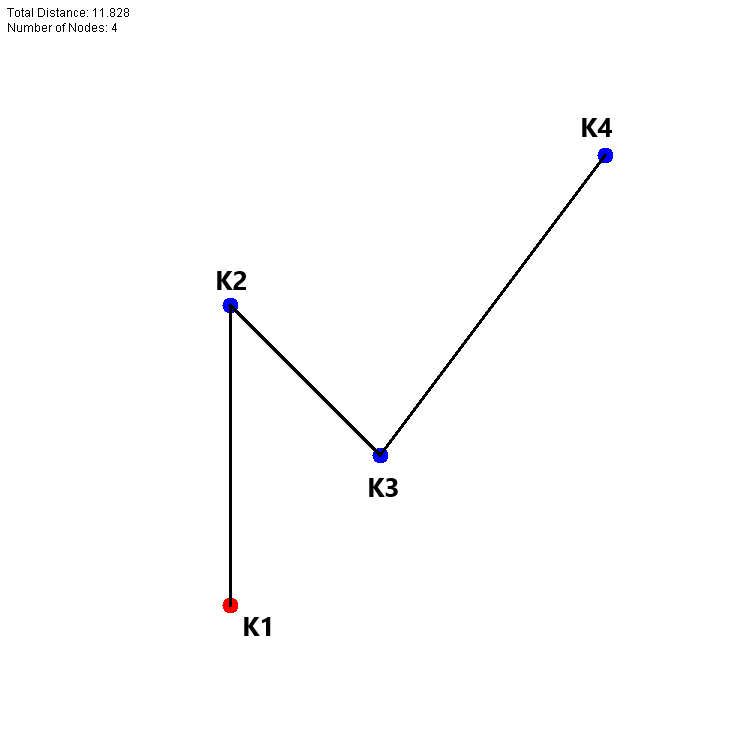
\includegraphics[width=0.35\textwidth]{Bilder/afterControl/after_control_ex1.PNG}
    }
    \hfil
    \subfloat[Verbesserter Graph \label{subfig:after-control-ex1-2}]{
        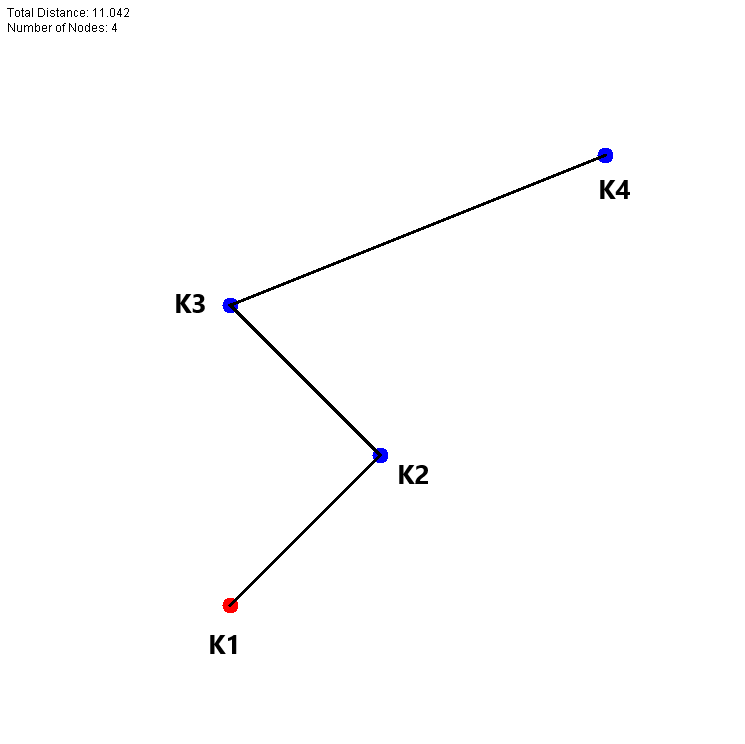
\includegraphics[width=0.35\textwidth]{Bilder/afterControl/after_control_ex2.PNG}
    }
    \end{center}
    \caption{Graph vor und nach der Nachbesserung}
    \label{fig:after-control-ex1}
\end{figure}

Das Beispiel in \vref{fig:after-control-ex1} zeigt einen Graphen mit einer initialen Knotenreihenfolge
$$P_{alt} = k_1,k_2,k_3,k_4$$
Durch das Umlegen zu
$$P_{neu} =k_1,k_3,k_2,k_4$$
erfolgt eine Verringerung der Gesamtdistanz.
Betrachtet man die hier betroffenen Kanten $E_1 = (k_1,k_2)$, $ E_2 = (k_1,k_3)$ und $E_3=(k_2,k_3)$ kann die Distanzverringerung anhand ihrer einzelnen Distanzen und ihres Auftretens in den beiden Graphen erklärt werden.
Da gilt 
$$E_1,E_3\in P_{alt} \textrm{ und } E_2,E_3 \in P_{neu}$$
kann eine Distanzverringerung mit
$$\omega(E_1) + \omega(E_3) < \omega(E_2) + \omega(E_3)$$
erklärt werden.
Im konkreten Beispiel in \vref{fig:after-control-ex1} drückt sich das durch eine Verringerung der Gesamtdistanz um 0,786\ac{LE} aus.


\subsection{Algorithmus zur Nachbesserung}
Ein Algorithmus, der Nachbesserung auf genau diese Art vornehmen soll, kann wie folgt vorgehen.
Betrachte beginnend mit dem zweiten Knoten in einem Pfad jeden Knoten.
Für jeden zu betrachteten Knoten wird jede Kante, an dessen Ende der aktuelle Knoten nicht steht, betrachtet.
Es gilt zu überprüfen, ob es für die Gesamtdistanz besser ist, wenn der aktuelle Knoten in die aktuelle Kante eingefügt wird.
Anders ausgedrückt: $p_i$ mit $i \geq 2,i\in\mathbb{N}$ sei ein Knoten in einem vollständigen Pfad mit $n$ Knoten und $n-1$ Kanten. Zusammen mit $p_i$ wird auch immer eine Kante $e_j=(p_{k-1},p_{k})$ betrachtet, sodass gilt $p_i \not \in e_j$.
Um nun zu überprüfen, ob es möglich ist eine Verbesserung des Graphs vorzunehmen wird überprüft ob 
$$\omega(p_{i-1},p_{i}) + \omega(p_{i},p_{i+1}) + \omega(e_j) > \omega(p_{i-1},p_{i+1}) + \omega(p_{k-1},p_i) + \omega(p_i,p_{k})$$
Ist dies der Fall wird die Reihenfolge der Knoten entsprechend geändert und $p_i$ zwischen $p_{i-1}$ und $p_{i+1}$ entfernt und zwischen $p_{k-1}$ und $p_k$ eingefügt. Wie genau das Einfügen in die Kante funktioniert kann in Algorithmus \vref{alg:after-control-merge} nachvollzogen werden.
\\\\
Eine vollständige Implementierung eines Algorithmus, der Verbesserung an einem bestehenden Graph vornimmt kann wie in Algorithmus \vref{alg:after-control} aussehen.
\begin{algorithm}[h]
    \caption{Nachbesserung eines Pfads}
    \label{alg:after-control}
    \begin{algorithmic}[1]
        \Require Pfad $P$
        \Require $P=p_1,p_2,\cdots,p_n,n>3,n\in \mathbb{N}$
        \For{$a\gets 2$, $a \leq n-1$, $a\gets a+1$}
            \For{$b \gets 3$, $b \leq n$, $b\gets b+1$}
                \If{$a=b$ \textbf{or} $a = b-1$}
                    \State \textsc{continue}
                \EndIf
                \If{$\omega(p_{a-1},p_{a}) + \omega(p_{a},p_{a+1}) + \omega(p_{b-1}, p_b) > \omega(p_{a-1},p_{a+1}) + \omega(p_{b-1},p_a) + \omega(p_a,p_{b})$}
                    \State $P \gets$ \textsc{resolve}($P, (p_{b-1}, p_b), p_a$)
                \EndIf
            \EndFor
        \EndFor\\
        \Return $P$

    \end{algorithmic}
\end{algorithm}
Damit beschreibt sich die Zeitkomplexität dieses Algorithmus mit 
$$f(n) = O(n^2)$$
Womit er, wie der Algorithmus \vref{alg:handle-crossover} Entfernen von Überkreuzungen, quadratisch zur Eingabemenge skaliert.




\chapter{Ergebnisse und Bewertung der verschiedenen Algorithmen}\label{sec:result}
Nachdem nun drei Algorithmen zur Generierung einer Route und zwei zu nachträglicher Überarbeitung vorgestellt wurden, gilt es nun Erkenntnisse über die Ergebnisse dieser Algorithmen im Vergleich zueinander zu gewinnen.
Dafür wurde ein Testszenario angelegt, in dem verschiedene Kombinationen dieser Algorithmen mehrmals getestet werden.
Jeder der drei Algorithmen zur Routengenerierung wird für sich, mit Auflösen von Überkreuzungen, mit Nachbesserung und mit Auflösen von Überkreuzungen und Nachbesserung getestet, wodurch es zwölf verschiedene Kombinationen gibt.
Diese Kombinationen werden $1\,000$ mal mit je $10,15,\cdots,100$ Knoten getestet und die Ergebnisse (Gesamtdistanz des finalen Graphs) vermerkt, wodurch $19\,000$ Datensätze entstehen. 
Wie aussagekräftigt diese Ergebnisse sind wird in dieser Arbeit nicht diskutiert.
\\
Tabelle \vref{tab:test-results1} zeigt die möglichen Kombinationen der vorgestellten Algorithmen, wie häufig eine Kombination die beste Lösung generiert hat und die Anteil der Kombination an den $19\,000$ besten Ergebnissen.
Eindeutig kann hier erkannt werden, dass -- unabhängig von der Strategie -- Routen, die nach Algorithmus \vref{alg:after-control} nachgebessert werden, den größten Teil der besten Lösungen beanspruchen.
Insgesamt erzielten die Kombinationen, die Nachbesserungs-Algorithmus anwenden $13\,083$ von $19\,000$ (68,86\%) besten Ergebnissen.
Den größten Teil macht dabei die Kombination, die den Insert-First-Algorithmus verwendet, aus.
Danach folgen, ebenfalls nur mit Nachbesserung, der Insert-Furthest-Algorithmus mit $4\,228$ und der Insert-Closest-Algorithmus mit $3\,648$ besten Ergebnissen.
Insgesamt verwenden 11,69\% der besten Lösungen nur einen Algorithmus zu Generierung des Graphen, 0,72\% lösen zusätzlich Überkreuzungen auf, 68,86\% verwenden den Algorithmus \vref{alg:after-control} zur Nachbesserung und 18,73\% beide dieser Verfahren.
Von den $19\,000$ besten Ergebnissen entfallen $7\,519$ (39,57\%) an eine Kombination mit dem Insert-First-Algorithmus, $5\,279$ (27,78\%) an den Insert-Closest-Algorithmus und $6\,202$ (32,64\%) an den Insert-Furthest-Algorithmus.
Weiterhin lässt sich aus den Datensätzen ablesen, dass die Differenz zwischen den Ergebnissen der besten und der schlechtesten Kombination mit zunehmender Knotenanzahl steigt.
Weicht die schlechteste Lösung bei 15 Knoten nur um 2,75\% von der Besten ab sind es bei 100 Knoten bereits 8,23\%.
\\
Zusätzlich kann festgestellt werden, dass Kombinationen, die sich bei der nachträglichen Überarbeitung nur auf das Entfernen von Überkreuzungen verlassen, einen sehr geringen Teil der besten Ergebnisse ausmachen.
Dies kann allerdings damit erklärt werden, dass wenn ein generierter Graph von Beginn an keine Überkreuzungen enthält, die Kombination ohne Ausbesserung dieser Überkreuzungen die gleiche Gesamtdistanz vorweist wie eine Kombination, die Überkreuzungen entfernt.
Ist dies der Fall wird nur erste Kombination gezählt.
\\\\
Um nun Aussagen darüber treffen zu können, welcher Algorithmus die besten Ergebnisse generiert muss zuerst eine Unterscheidung getroffen werden.
Definiert man die beste Algorithmenkombination nach der Anzahl der besten Ergebnisse, so ergibt die Kombination von Insert-First und Nachbesserung als beste Kombination,
Wird jedoch die durchschnittliche Gesamtdistanz der generierten Routen als Maßstab gewählt, ist die beste Kombination die von Insert-First, Nachbesserung und dem Entfernen von Überkreuzungen.\footnote{Diese Ergebnisse leiten sich von den in \textit{data.xlsm} aufgeführten Testergebnissen ab, auffindbar in dem in der Einleitung angemerktem GitHub Repository}
Beide diese Ergebnisse stehen jedoch gegen die gestellten Erwartungen, da in \vref{sec:insert-closest-verfahren} und \vref{sec:insert-furthest-verfahren} versucht wurde den Insert-First-Algorithmus zu verbessern.

Nach Auswertung der Daten scheint es aber so, als seien die Ergebnisse der Variationen des Insert-First-Verfahrens insgesamt schlechter als die des ursprünglichen Algorithmus.
Vergleicht man die durchschnittlichen Ergebnisse des Insert-First-Algorithmus in Kombination mit dem Nachbesserungs-Algorithmus mit den besten Durchschnittswerten aller Kombinationen, kann festgestellt werden, dass diese Kombination durchschnittlich 0,49\% vom besten Durchschnitt abweicht, sofern sie nicht selbst die beste Lösung generiert.



\begin{center}
    \begin{table}
        \begin{tabular}{ l | l | l | l | l }
            \textbf{Strategie} & \textbf{Überkreuzungen} & \textbf{Nachbesserung} & \textbf{\# Beste} & \textbf{\% Beste} \\ \hline
            First & Nein & Nein & $1\,024$ & 5,39\% \\
            First & Nein & Ja & $5\,207$ & 27,41\% \\
            First & Ja & Nein & $51$ &  0,27\% \\
            First & Ja & Ja & $1\,237$ & 6,51\% \\ \hline
            Furthest & Nein & Nein &  481 & 2,53\% \\
            Furthest & Nein & Ja & $4\,228$ & 22,25\% \\
            Furthest & Ja & Nein & 44 & 0,23\% \\
            Furthest & Ja & Ja & $1\,449$ & 7,63\% \\ \hline
            Closest & Nein & Nein & 717 & 3,77\% \\
            Closest & Nein & Ja & $3\,648$ & 19,20\% \\
            Closest & Ja & Nein & 41 & 0,22\% \\
            Closest & Ja & Ja & 873 & 4,59\% \\ \hline
        \end{tabular}
        \caption{Beste Testergebnisse nach verwendeten Algorithmen}
        \label{tab:test-results1}
    \end{table}
\end{center}

% TODO: neu schreiben und
% Beste einzelergebnisse?
% Konsistent gute ergebnisse

\chapter{Zusammenfassung und Ausblick}
% \chapter{Literaturverzeichnis}

%	Anleitungs-Datei anleitung.tex einziehen. Auf diese Weise sollten Sie versuchen, für jedes einzelne
% Kapitel eine eigene Datei anzulegen und mittels input-Kommando einzuziehen.
% % !TEX root =  master.tex
\chapter{Gebrauchsanleitung}

\section{Übersicht über die Vorlage}
Die Vorlage wurde im UTF-8 Encoding erstellt. Sollten daher z.\,B. Umlaute in Ihrem \LaTeX-Editor nicht korrekt dargestellt werden, überprüfen Sie bitte die Encoding-Ein\-stel\-lun\-gen des Editors. In seltenen Fällen müssen Sie die Vorlage danach noch einmal neu in den Editor einbinden. 
Die Vorlage beinhaltet die folgenden, in Tabelle \vref{tab:dateien} aufgelisteten Dateien: 
\begin{table}[h!]
	\centering
\begin{tabular}{lp{10cm}}
	\textbf{Dateiname} & \textbf{Beschreibung}\\\toprule
	\texttt{master.tex} & Die Hauptdatei. Alle anderen Dateien werden von dieser Datei eingezogen. \\
	\texttt{abstract.tex} & Die Kurzfassung der Arbeit. \\	
	\texttt{config.tex} & Konfigurationseinstellungen 	 der einzelnen Pakete\\
	\texttt{acronyms.tex} & Definition von Abkürzungen. \\
	\texttt{titlepage.tex} & Titelseite der Arbeit. \textbf{Bitte Anpassen!}\\
	\texttt{anleitung.tex} & Diese Anleitung\\ 
	\texttt{bibliography.bib}&  Die Literaturdatenbank -- hier können Sie die verwendete Literatur einpflegen.\\
	\texttt{ewerkl.tex} & Ehrenwörtliche Erklärung. \textbf{Bitte Anpassen!}\\
	\texttt{appendix.tex} & Anhang bzw. Anhänge \\\bottomrule
\end{tabular}
\caption{\label{tab:dateien}Übersicht über die Dateien der Vorlage}
\end{table}

Es werden -- unter anderem -- die folgenden Zusatzpakete von dieser Vorlage eingezogen und sollten daher in aktuellen Versionen installiert sein: 
\begin{itemize}
	\item\texttt{KOMA-Script} bzw. die Dokumentenklasse \texttt{scrreprt}
	\item\texttt{hyperref} für PDF-Informationen und Links 
	\item \texttt{babel} für länderspezifische Einstellungen
	\item \texttt{csquotes} für sprachabhängige Anführungszeichen (Befehl: \texttt{\textbackslash enquote})
	\item \texttt{acronym} für das Erstellen des Abkürzungsverzeichnisses 
	\item \texttt{booktabs} für das typografisch schöne Setzen von Tabellen 
	\item \texttt{varioref} für einfaches Referenzieren 
	\item \texttt{listings} für schöne Quelltexte
	\item \texttt{algorithm} für schöne Algorithmen
	\item \texttt{bibltatex} und \texttt{biber} für die Erstellung des Literaturverzeichnisses.
\end{itemize}
Alle Konfigurationen dieser Vorlage können in der Datei \texttt{config.tex} eingesehen und ggf. verändert werden. Bitte schauen Sie sich die entsprechenden Dokumentationen 
der Pakete an (\url{https://www.ctan.org}), um deren Verwendung und Möglichkeiten jenseits der hier gezeigten Beispiele zu erlernen.


\section{Übersetzung von \LaTeX-Dateien}
Die Übersetzung von \LaTeX-Dateien erfolgt in mehreren Schritten und unter der Zuhilfenahme unterschiedlicher Programme. Das Hauptdokument (hier die Datei \texttt{master.tex}) wird mittels \texttt{pdflatex} zu einem PDF übersetzt. Ggf. ist eine mehrfache Übersetzung notwendig, um z.\,B. das Inhaltsverzeichnis korrekt darzustellen. 

Für die Einbindung des Literaturverzeichnisses wird nicht mehr das ältere \texttt{bibtex}, sondern das neuere \texttt{biber} in Kombination mit \texttt{biblatex} verwendet. Bitte stellen Sie Ihren \LaTeX-Editor so ein, dass die Verwendung von Biber beim Übersetzungsprozess erfolgt. 

\section{Verwendung von Akronymen}
Akronyme müssen in der Datei \texttt{acronyms.tex} definiert werden (schauen Sie sich hierzu bitte die entsprechende Paket-Dokumentation an!)
Ein definiertes Akronym kann dann mit dem Befehl \texttt{\textbackslash ac} verwenden, so wird z.\,B. \texttt{\textbackslash ac\{DHBW\}} zu \ac{DHBW}. Im weiteren Verlauf wird das 
Acronym dann nur noch in der Kurzform dargestellt: \ac{DHBW}. Die Aufnahme eines verwendeten Akronyms in das Abkürzungsverzeichnis erfolgt automatisch. \autocite[Vgl.][S. 77ff]{TestOnlineQuelle}\autocite[Vgl.][S. 42]{ME12}

\section{Zitieren von Quellen}
Mit dem Befehl \texttt{\textbackslash autocite} kann zitiert werden, z.\,B. so. \autocite[Vgl.][S. 18ff.]{ME12} Sollen mehrere Referenzen auf einmal gesetzt werden, können Sie dies mit dem Befehl \texttt{\textbackslash autocites} erreichen, z.\,B. so\autocites[Vgl.][S. 10]{ME12}[][S. 100]{TD15}. Wird \texttt{autocite} konsequent 
verwendet, kann in der Datei \texttt{config.tex} der Zitationsstil umgeschaltet werden, ohne dass im Text Veränderungen vorgenommen werden müssen. Vorkonfigurierte Stile sind Alphabetic, Harvard, Fußnotenzitat und IEEE-Style. Die Übernahme der Quellen in das Literaturverzeichnis erfolgt automatisch. Ein Beispiel für eine Online-Quelle ist ebenfalls enthalten.\autocite[Vgl.][]{TestOnlineQuelle}




Soll einer Abbildung eine Quellenangabe zugefügt werden, bietet es sich an, diese direkt in der jeweiligen Abbildungsbeschriftung zu hinterlegen. Hierfür kann der Befehl \texttt{\textbackslash cite} verwendet werden, um eine ungewollte Fußnote zu vermeiden. Ein Beispiel ist in Abbildung 
\vref{fig:test} zu sehen. 


\section{Text in Anführungszeichen}
Soll ein Text in Anführungszeichen gesetzt werden, kann dies über den Befehl \texttt{\textbackslash enquote} \enquote{so erreicht werden}. Die Anführungszeichen ändern sich automatisch auf die 
jeweiligen Länderspezifika, wenn die Spracheinstellung des \texttt{babel}-Pakets geändert wird. Voreinstellung ist die deutsche Verwendung von 
Anführungszeichen.




\section{Beispiele}
\lipsum[1]

\subsection{Unterabschnitte}
Es gibt neben \texttt{\textbackslash chapter} auch noch  \texttt{\textbackslash section}, \texttt{\textbackslash subsection}, \texttt{\textbackslash subsubsection} etc. Eine zu starke Untergliederung des Textes sollte jedoch vermieden werden (z.\,B. ein Abschnitt 3.4.2.5.3). 

\subsection{Tabellen und Abbildungen}
Tabellen und Abbildungen sind sogenannte \textit{Floating Objects}, d.\,h. \LaTeX\ setzt diese Objekte an Positionen, die satztechnisch geeignet sind. Daher kann es vorkommen, dass Tabellen oder Abbildungen auf einer anderen Seite erscheinen, die dann referenziert werden müssen. Hier ein Beispiel dafür: 

In Tabelle \vref{tab:tabelle1} ist eine Tabelle abgebildet, die mit dem Befehl \texttt{\textbackslash vref} referenziert wurde. Gleiches kann man auch mit Abbildungen 
machen, wie z.\,B. mit der Abbildung \vref{fig:test}. \LaTeX~ kümmert sich darum, wo die Abbildungen gesetzt werden und passt den Text der Referenz entsprechend an. Soll nur die Nummerierung in den Text geschrieben werden, dann kann auch der Befehl \texttt{\textbackslash ref} verwendet werden.
Abbildungen sollten -- falls möglich -- als Vektor-PDF eingebunden 
werden, da die diese dann beliebig skalieren können.

\lipsum[1]
\begin{table}
	\centering
	\begin{tabular}{p{3cm}crl}
		\textbf{Spalte 1} & \textbf{Spalte 2} & \textbf{Spalte 3} & \textbf{Spalte 4}\\\toprule
		Zeile 1 Spalte 1 &  Zeile 1 Spalte 2 & Zeile 1 Spalte 3 & Zeile 1 Spalte 4\\
		Zeile 2 Spalte 2 &  Zeile 2 Spalte 2 & Zeile 2 Spalte 3 & Zeile 2 Spalte 4\\\midrule
		Zeile 3 Spalte 1 &  Zeile 3 Spalte 2 & Zeile 3 Spalte 3 & Zeile 3 Spalte 4\\
		Zeile 4 Spalte 1 &  Zeile 4 Spalte 2 & Zeile 4 Spalte 3 & Zeile 4 Spalte 4\\\bottomrule
	\end{tabular}
	\caption[Testtabelle]{\label{tab:tabelle1}Testtabelle}
\end{table}
\lipsum[1-2]

\begin{figure}
	\centering 
	
\includegraphics{img/firmenlogo.jpg}
	\captionsetup{format=hang}
	\caption[Optionaler Kurztitel für das Abbildunggsverzeichnis]{\label{fig:test}Demo-Abbildung, um zu verdeutlichen, wie gleitende Objekte gesetzt werden und wie entsprechend die Quelle zitiert wird. \\Quelle: \cite[][S. 223]{TD15}}
\end{figure}
	
\subsection{Listings}	

Das Einbinden eines Listings mit der entsprechenden Umgebung ist auch kein Problem, wie man in Listing \vref{lst:helloworld} sehen kann. Schauen Sie sich hierzu das \texttt{listings}-Paket an! 
		
		\newpage
		
		
\lstset{language=Java}
\begin{lstlisting}[caption={Hello World!}, label={lst:helloworld}]
public static void main(String args[]) {
   System.out.println("Hello World!");
}
\end{lstlisting}


\subsection{Mathematische Formeln}
Auch mathematische Ausdrücke können mit \LaTeX~ sehr gut gesetzt werden, wie man anhand der Gleichungen \vref{eqn:e1} und \vref{eqn:e2} sehen kann -- konsultieren Sie hierzu bitte entsprechende Dokumentationen, die Online zur Verfügung stehen.
\begin{equation}
\left|{1\over N}\sum_{n=1}^N \gamma(u_n)-{1\over 2\pi}\int_0^{2\pi}\gamma(t){\rm d}t\right| \le {\varepsilon\over 3}.\\
\label{eqn:e1}
\end{equation}

\begin{equation}
f(x)=x^2
\label{eqn:e2}
\end{equation}


\subsection{Algorithmen}
Algorithmen können als Pseudocodes dargestellt und referenziert werden, wie z.\,B. in Algorithmus \vref{alg:euclid} -- sogar bis auf Zeilennummern
(siehe die \texttt{while}-Anweisung in Zeile \vref{alg:euclid:while}). Schauen Sie sich hierzu bitte das Paket \texttt{algorithmicx} an.



\begin{algorithm}
\begin{algorithmic}[1]
\Procedure{Euclid}{$a,b$}\Comment{The g.c.d. of a and b}
   \State $r\gets a\bmod b$
   \While{$r\not=0$}\Comment{We have the answer if r is 0} \label{alg:euclid:while}
      \State $a\gets b$
      \State $b\gets r$
      \State $r\gets a\bmod b$
   \EndWhile\label{euclidendwhile}
   \State \textbf{return} $b$\Comment{The gcd is b}
\EndProcedure
\end{algorithmic}
\caption{Euklid'scher Algorithmus}\label{alg:euclid}
\end{algorithm}



%	Literaturverzeichnis
\printbibliography[title=Literaturverzeichnis]
\cleardoublepage

% Der Anhang beginnt hier - jedes Kapitel wird alphabetisch aufgezählt. (Anhang A, B usw.)
\appendix
\ihead{\appendixname~\thechapter} % Neue Header-Definition

% appendix.tex einziehen
\chapter{Anhang}
\section{Bilder}
% TODO: Bilder insertFirst Good (4)
% TODO: Bilder insertFirst Bad (4)
% TODO: Bilder insertFurthest Good (5)
% TODO: Bilder insertFurthest Bad (5?)
% TODO: Merge Algorithmus in Anhang


% \section{Subtestanhang}

% \chapter{Noch ein Testanhang}

% -------------------------------------------------------------- 
% INSERT CLOSEST BAD COMPLETE
\begin{figure}[H]
    \begin{center}
        \subfloat[$m = 2$\label{app:subfig:insert-closest-BAD-m1}]{%
        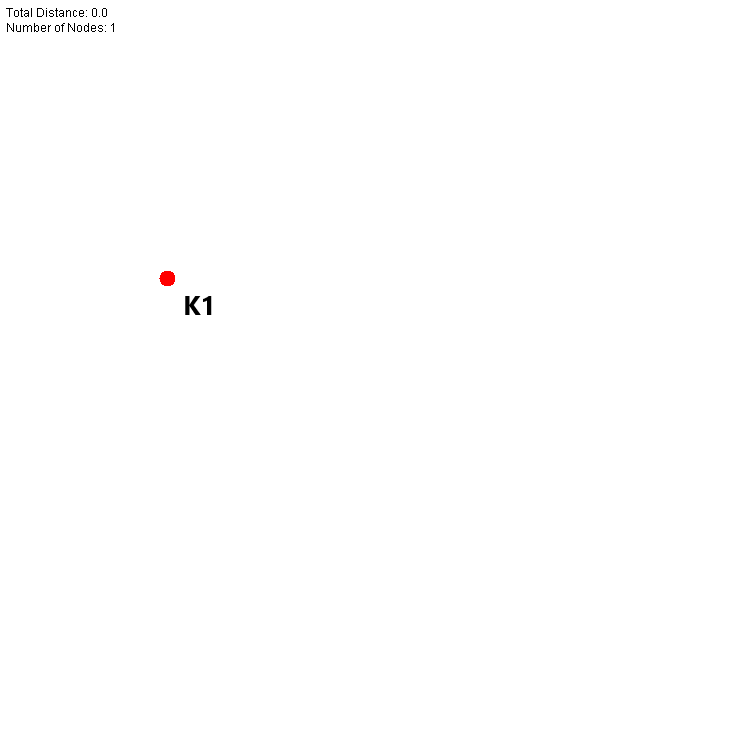
\includegraphics[width=0.6\textwidth]{./Bilder/insertClosest/insert_closest_ex_BAD_1.PNG}
        }
    \end{center}
    \phantomcaption
\end{figure}
\begin{figure}[H]\ContinuedFloat
    \begin{center}
        \subfloat[$m = 3$\label{app:subfig:insert-closest-BAD-m2}]{%
        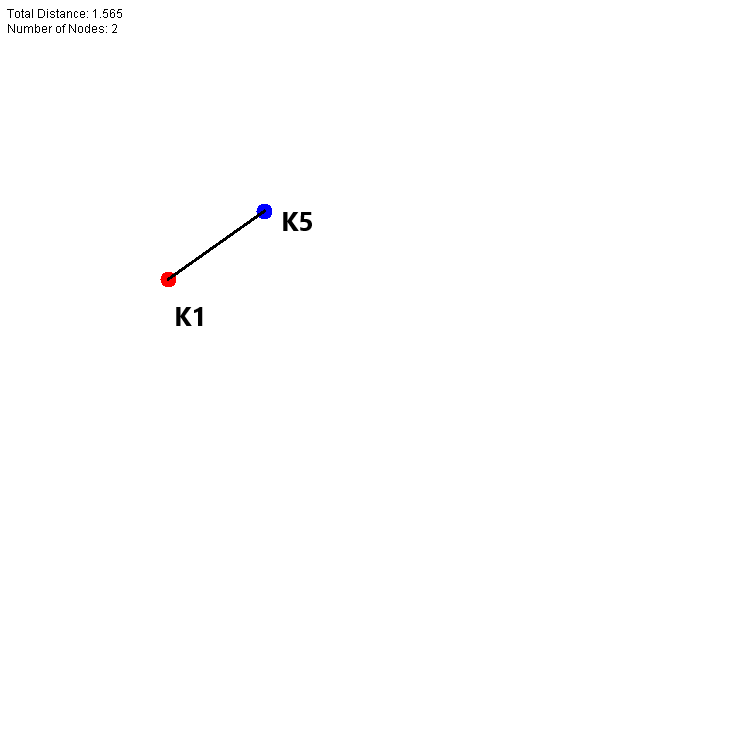
\includegraphics[width=0.6\textwidth]{./Bilder/insertClosest/insert_closest_ex_BAD_2.PNG}
        }
    \end{center}
    \phantomcaption

\end{figure}
\begin{figure}[H]\ContinuedFloat
    \begin{center}
        \subfloat[$m = 4$\label{app:subfig:insert-closest-BAD-m3}]{%
        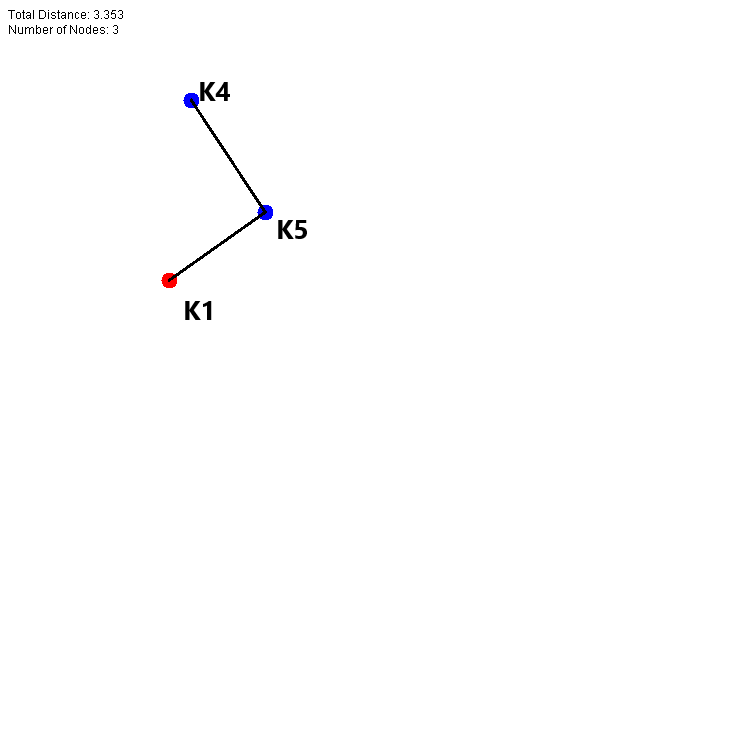
\includegraphics[width=0.6\textwidth]{./Bilder/insertClosest/insert_closest_ex_BAD_3.PNG}
        }
    \end{center}
    \phantomcaption

\end{figure}
\begin{figure}[H]\ContinuedFloat
    \begin{center}
        \subfloat[$m = 5$\label{app:subfig:insert-closest-BAD-m4}]{%
        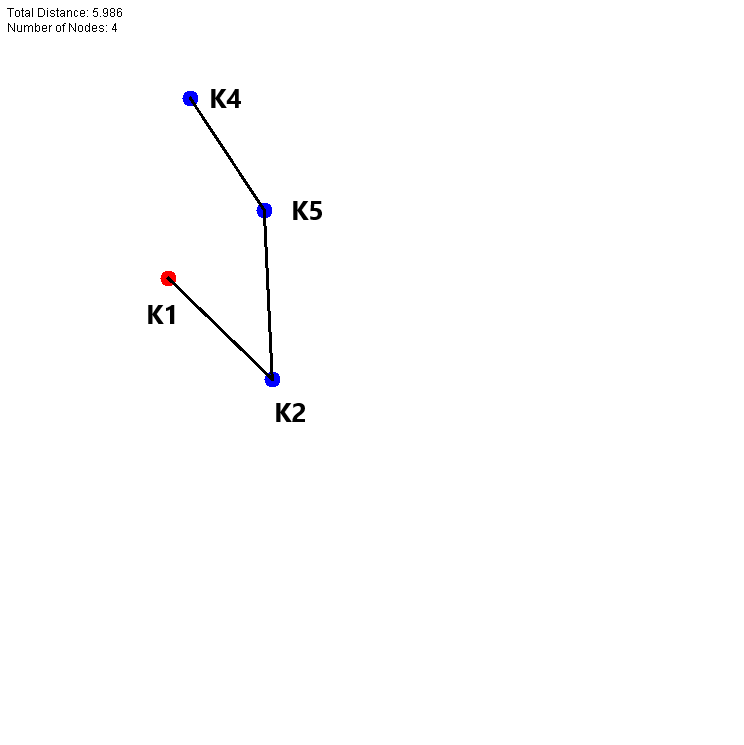
\includegraphics[width=0.55\textwidth]{./Bilder/insertClosest/insert_closest_ex_BAD_4.PNG}
        }
    \end{center}
    \phantomcaption

\end{figure}
\begin{figure}[H]\ContinuedFloat
    \begin{center}
        \subfloat[$m = 5$\label{app:subfig:insert-closest-BAD-m5}]{%
        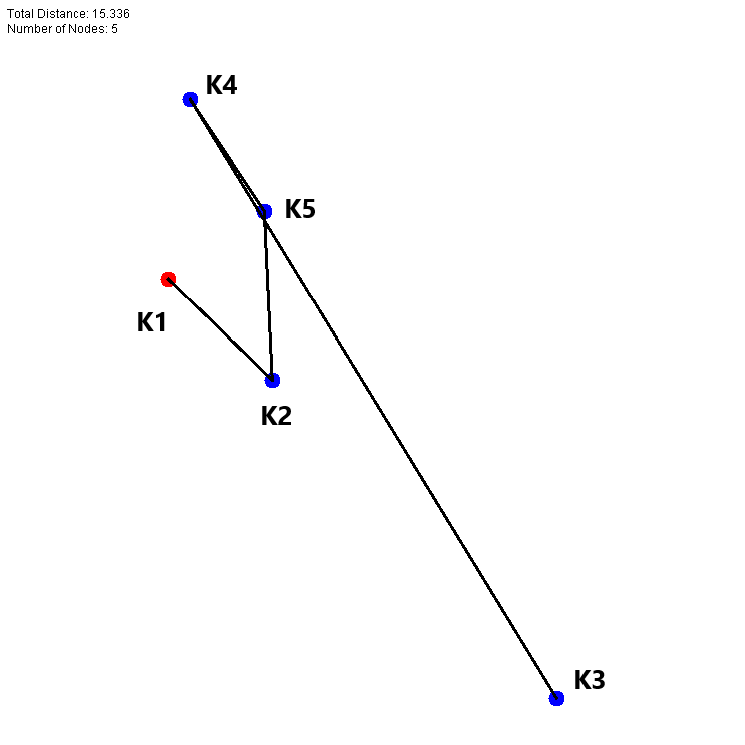
\includegraphics[width=0.55\textwidth]{./Bilder/insertClosest/insert_closest_ex_BAD_5.PNG}
        }
    \end{center}
    \caption{Viele Bilder}
    \label{app:fig:insert-closest-BAD-complete}
\end{figure}


% -------------------------------------------------------------- 
% Crossover Example 40 Nodes
\begin{figure}[H]
    \begin{center}
        \subfloat[Pfad mit einem Crossover\label{app:subfig:40-nodes-with-crossover}]{%
        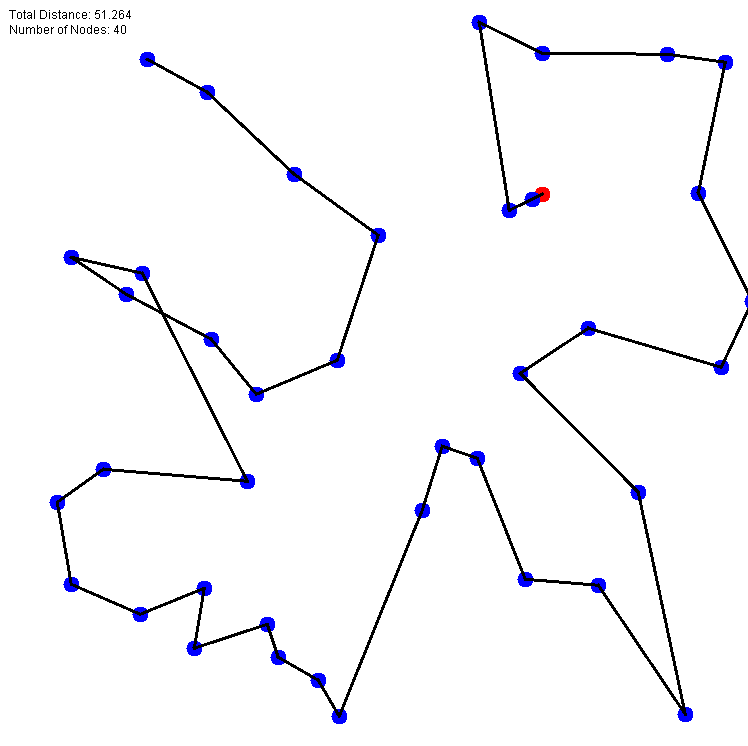
\includegraphics[width=0.55\textwidth]{./Bilder/crossover/40_nodes_with_crossover}
        }
    \end{center}
    \phantomcaption

\end{figure}
\begin{figure}[H]\ContinuedFloat
    \begin{center}
        \subfloat[Pfad mit aufgelöstem Crossover\label{app:subfig:40-nodes-without-crossover}]{%
        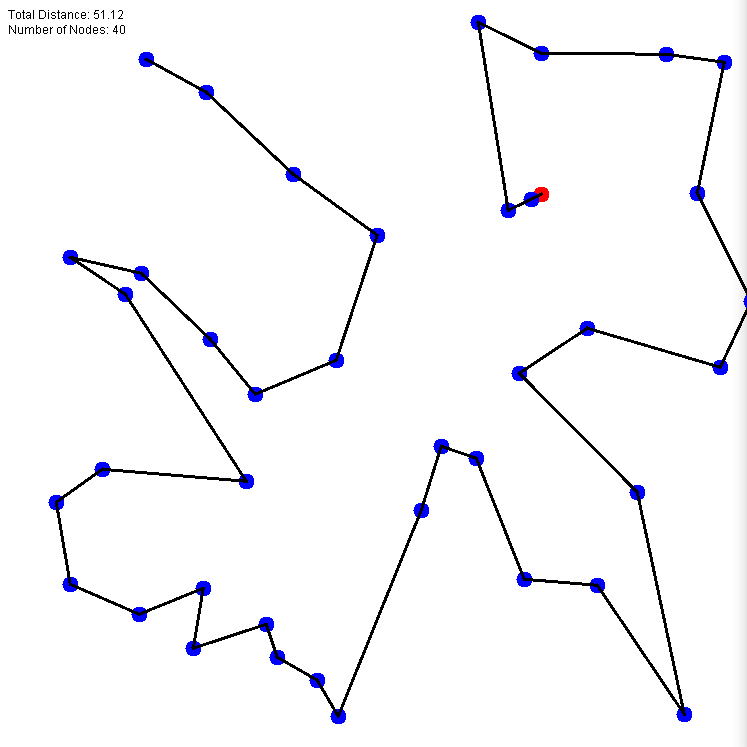
\includegraphics[width=0.55\textwidth]{./Bilder/crossover/40_nodes_without_crossover.PNG}
        }
    \end{center}
    \caption{Pfad aus 40 Knoten mit und ohne Crossover}
    \label{app:fig:40-nodes-crossover-example}
\end{figure}

% -------------------------------------------------------------- 
% After Control Example 40 Nodes

\begin{figure}[H]
    \begin{center}
        \subfloat[Teilpfad vor Nachbesserung\label{app:subfig:40-nodes-before-after-control}]{
            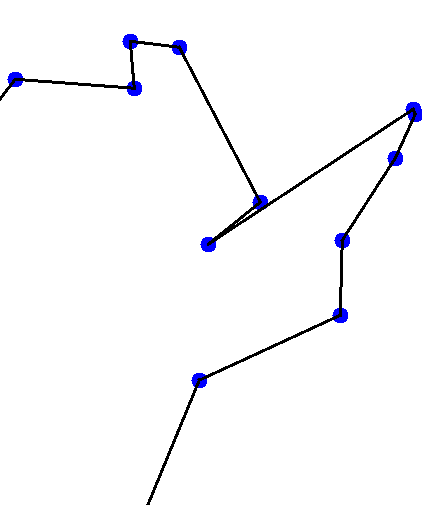
\includegraphics[width=0.3\textwidth]{Bilder/afterControl/before_after_control.PNG}
        }
    \end{center}
    \phantomcaption

\end{figure}

\begin{figure}[H]\ContinuedFloat
    \begin{center}
        \subfloat[Teilpfad nach Nachbesserung\label{app:subfig:40-nodes-after-after-control}]{
            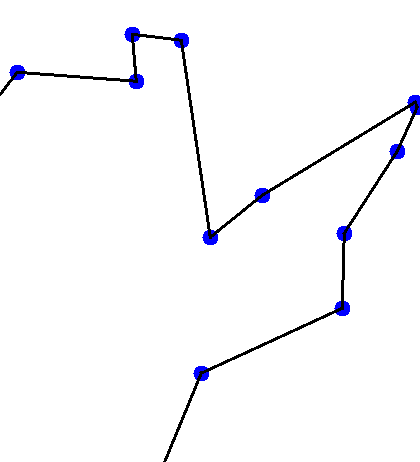
\includegraphics[width=0.3\textwidth]{Bilder/afterControl/after_after_control.PNG}
        }
    \end{center}
    \caption{Beispiel für eine Nachbesserung, Teilpfad}
\end{figure}

\section{Algorithmen}
\begin{algorithm}
    \caption{Einfügen eines neuen Knoten in einen Pfad}
    \label{alg:merge-node-into-path}
    \begin{algorithmic}[1]
        \Require Pfad $P = p_1,\ldots,p_n$ mit $\forall p \in G$
        \Comment Jedes p ist Knoten in Graph $G$
        \Require Knoten $K^*$, Index $i$, $i \leq n + 1$
        \Comment neuer Knoten $K^*$, einzufügen an Index $i$
        \For{$a \gets n$, $a \geq i$, $a \gets a+1$}
            \State $p_{a+1} \gets p_a$
        \EndFor
        \State $p_i \gets K^*$ \\
        \Return $P$
    \end{algorithmic}
\end{algorithm}

\begin{algorithm}
    \caption{Tauschen von Knoten auf einem Graph zwischen zwei eingegebenen Knoten}
    \label{alg:swap-nodes-inbetween}
    \begin{algorithmic}[1]
        \Require Graph $G$, Knotenpaare $A_1,A_2$ und $B_1,B_2$
        \Require $G=k_1,k_2,\cdots,k_n$, $n>4$
        \State $i_{A_2} \gets$ \textsc{index}($A_2$)
        \State $i_{B_1} \gets$ \textsc{index}($B_1$)
        \If{$i_{A_2} > i_{B_1}$}
            \State \textsc{swap}($i_{A_2}$, $i_{B_1}$) 
            \Comment \textsc{swap} weißt beiden Parametern den Wert des anderen zu
        \EndIf
        \While{$i_{A_2} < i_{B_1}$}
            \State \textsc{swap}($k_{i_{A_2}}$,$k_{i_{B_1}}$)
        \EndWhile
    \end{algorithmic}
\end{algorithm}

\begin{algorithm}
    \caption{Berechnung der Distanz zwischen zwei Knoten}
    \label{alg:calc-distance-two-nodes}
    \begin{algorithmic}[1]
        \Require Knoten $A$, Knoten $B$
        % \Require $P=p_1,\cdots,\p_n$, $n \geq 2$
        \State $d \gets \sqrt{|x_A - x_B|^2 + |y_A - y_B|^2}$\\
        \Return $d$
        % \State 
    \end{algorithmic}
\end{algorithm}

\begin{algorithm}
    \caption{Berechnung der Gesamtdistanz eines Pfads}
    \label{alg:calc-total-distance}
    \begin{algorithmic}[1]
        \Require Pfad $P$
        \Require $P=p_1,\cdots,p_n$, $n \geq 2$
        \State sum $\gets 0$
        \For{$a \gets 2$, $a \leq n$, $a \gets a + 1$}
            \State sum $\gets sum + \textrm{\textsc{distance}}(p_{a-1}, p_a)$
        \EndFor\\
        \Return sum
        % \State 
    \end{algorithmic}
\end{algorithm}


\begin{algorithm}
    \caption{Einfügen eines Knotens in eine Kante}
    \label{alg:after-control-merge}
    \begin{algorithmic}[1]
        \Require Pfad $P$, Kante $e_j$ und Knoten $p_i$
        \Require $P=p_1,p_2,\cdots,p_n,e_j=(p_{k-1},p_k),n>3,k>1n,i,j,k\in \mathbb{N}$
        \If{i < k}
            \For{$a\gets i+1, a < k, a \gets a + 1$}
                \State \textsc{swap}($p_i,p_a$)
            \EndFor
        \Else
            \For{$a\gets i, a > k - 1, a \gets a - 1$}
                \State \textsc{swap}($p_i,p_a$)
            \EndFor
        \EndIf\\
        \Return $P$
    \end{algorithmic}
\end{algorithm}


% Ehrenwörtliche Erklärung ewerkl.tex einziehen
% !TEX root =  master.tex

\clearpage
\chapter*{Ehrenwörtliche Erklärung}

% Wird die folgende Zeile auskommentiert, erscheint die ehrenwörtliche
% Erklärung im Inhaltsverzeichnis.

% \addcontentsline{toc}{chapter}{Ehrenwörtliche Erklärung}
Ich versichere hiermit, dass ich die vorliegende Arbeit
 mit dem Thema: \textit{\DerTitelDerArbeit} selbstständig verfasst und keine anderen als die angegebenen Quellen und
Hilfsmittel benutzt habe. Ich versichere zudem,
dass die eingereichte elektronische Fassung mit der gedruckten Fassung übereinstimmt.

\vspace{3cm}
Ort, Datum \hfill \DerAutorDerArbeit



\end{document}
